
The work presented here develops an analysis of English \textit{otherwise}, drawing on tools from the dynamic semantics and information structural literatures.\footnote{This chapter represents a (very lightly modified) version of a manuscript emerging out of joint work with Dr Hadas Kotek. As of \today, that manuscript is under review for \textit{Journal of Semantics} (ID \texttt{JS-19-09-088.R1}).} A simple example is given in (\nextx): 

\pex  \textit{A simple \emph{`otherwise'} sentence and a paraphrase of its meaning}:
\a  Mary wears a yellow vest when she cycles.\\\-\hfill \textit{Otherwise}, drivers might not see her on the road.
\a  \color{violet}$\approx$ \uline{If} Mary does \uline{not} wear a yellow vest, drivers might not see her. \xe
\color{black}

As (\lastx) illustrates, \textit{otherwise} can be paraphrased as a conditional: its antecedent is the \textit{negation} of the sentence preceding it, and its consequent is the sentence following it. A first approximation of this intuition can be spelled out as in (\nextx): 
%


\pex  \textit{A first attempt at the meaning of \emph{otherwise}:}\hfill (to be revised)
$$\llbracket  \textit{otherwise} \rrbracket=\lambda p_{ \langle s,t\rangle}\lambda q_{\langle s,t\rangle}\lambda w_s.\neg p(w)\to q(w)$$
Given two propositions $ p,q $ and some world $ w $, \textit{otherwise} states that, if $ p $ doesn't hold in $ w $, then $ q $ holds in $ w $.\xe


In this paper, we focus on \textit{otherwise}'s use as a discourse `connective' or `anaphor' \citep[e.g.][]{Webber2001, Kruijff-Korbayova2001}, so named because of its apparent interpretive reliance on foregoing elements of discourse.\footnote{For the purposes of this current paper, we restrict our attention to these ``inter-clausal'' adverbial uses. As we will discuss in \S\ref{sec:conclusion}, however, we anticipate that our account could be expanded to account for other uses as well.}  This is demonstrated by the sentence pair (\nextx), from \citet[7]{Webber2001}. Each sentence is accompanied by a paraphrase that spells out its intended meaning.


\pex \label{redlightR} \textit{``Red  Light sentences'' with the discourse anaphor \emph{`otherwise'}}:\footnotemark{}
\a  If the light is red, stop. \textit{Otherwise} go straight on.\\
\color{violet}\phantom{If the light is } $\approx$ If the light is \ul{not} red\ldots \label{redlighta}
\color{black}
\vspace{.5\baselineskip}
\a  If the light is red, stop. \textit{Otherwise} you'll get a ticket.\\
\color{violet}\phantom{If the light is } $\approx$ If the light is red and you \ul{don't} stop\ldots \label{redlightb}
\color{black}\xe

\footnotetext{In section \ref{sec:red-light-analysis}, we identify a \textit{third}, previously unnoticed reading of this sentence: 
	\pex  If the light is red, stop. \textit{Otherwise} there'll be chaos on the roads.\\
	\color{violet}\phantom{If the light} $\approx$ If the rules of traffic \ul{aren't} obeyed\ldots 
	\color{black}\xe
	
	At this point in the paper, however, our points can be made by concentrating on the two cited variants in \ref{redlightR} which have been recognized in previous literature.} %fn

As example \ref{redlightR} makes clear, the question of how to determine the antecedent to \textit{otherwise} is quite subtle. While the pronounced utterance preceding \textit{otherwise} is identical in both \ref{redlighta} and \ref{redlightb}, it is clear that the proposition that is interpreted as the antecedent of \textit{otherwise} in each case is different. How, then, is this antecedent determined? It is clear that some pragmatic means must be in play.

In a nutshell, we develop an analysis of \textit{otherwise} which draws on existing dynamic semantic analyses of conditionals. We'll argue that \textit{otherwise} contributes a discourse move whose content is to predicate a subsequent proposition of the \textit{complement} of some	set of worlds computed based on the clause preceding \textit{otherwise}. This will allow us to predict the set of possible antecedents to \textit{otherwise} in a given sentence, how a particular antecedent is chosen out of this set, and how it is constrained. 

At this point, it is important to be clear about the terminology and assumptions that we will adopt in this paper. As example \ref{redlightR} demonstrates, the \textit{antecedent utterance} preceding \textit{otherwise} need not be identical to the \textit{antecedent proposition} used in the interpretation of \textit{otherwise}, although, as we will show, the former informs and constrains the latter. In fact, the antecedent utterance need not be a proposition at all: it can be a conditional or a question, as well: 

\pex  \label{antecedent-type}\textit{\emph{Otherwise}'s antecedent utterance may be a declarative, imperative, or (certain) interrogatives:}
\a  Jake's asleep, \textit{otherwise} he would have come.
\a  Stop. \textit{Otherwise} you'll get a ticket.
\a  Do you have your car? \textit{Otherwise} I'll give you a lift.
\a  Do you want to get a beer at Three Sheets or Counterweight tonight? \textit{Otherwise} you make a bloody suggestion.\xe
\footnote{To our ears, (d) can be read with either polar question or alternative question intonation. In both cases, a proposition of the form `you don't want to get a beer at either place' seems to be accommodated.} %fn 

A (declarative) \textit{otherwise} statement, then, includes three components: (a) An \textit{antecedent utterance} is put on the table as accurate to the best of the speaker's knowledge.\footnote{That is, \textit{asserted}, cf. \citealt{Stalnaker1979}.} (b) An \textit{antecedent proposition} is accommodated, representing the complement of a set of worlds introduced by this antecedent utterance.\footnote{We focus predominantly on declarative antecedents in this paper, but we believe that future work should lead to interesting discoveries about the shape of possible non-declarative antecedents and the accommodation step we describe here.} %fn 
(c) The \textit{consequent} of \textit{otherwise} provides a description of what happens in such worlds.\footnote{Syntactically, we believe that only the \textit{consequent} clause is an argument of \textit{otherwise}. The \textit{antecedent} that \textit{otherwise} operates on is an accommodated pragmatic object, and we do not make a claim about its syntactic form. This might suggest that the term \textit{prejacent} is more appropriate here. However, since we build heavily on the semantics of conditionals, and believe that \textit{otherwise} relates two propositions to one another, we choose terminology that aligns with these theoretical choices.} %fn 
We spell this out below for examples \ref{redlighta} and \ref{redlightb}:

\pex \textit{Components of the \emph{otherwise} sentence in \ref{redlighta}:}
\a  Antecedent utterance: \textit{If the light is red, stop.} \label{components1-a}
\a  Antecedent proposition: \textit{The light is not red.} \label{components1-b}
\a  Consequent: \textit{(You) go straight on.} \label{components1-c}\xe

\pex \textit{Components of the \emph{otherwise} sentence in \ref{redlightb}:}
\a  Antecedent utterance: \textit{If the light is red, stop.} \label{components2-a}
\a  Antecedent proposition: \textit{The light is red and you don't stop.} \label{components2-b}
\a  Consequent: \textit{You get a ticket.} \label{components2-c}\xe

%Pragmatically speaking, the consequent is often taken to represent a \textit{justification} for the antecedent proposition, providing a discourse link between these two components. Here: if the light is \uline{not} red \ref{components-b}, go straight on \ref{components-c}.
%
%HK: commented out because this comes up again in section 2 and disrupts the flow here.

The \textit{antecedent propositions} in \ref{components1-b} and \ref{components2-b} are different, but we see that they are both derived from the same \textit{antecedent utterance}, \ref{components1-a} = \ref{components2-a}. More specifically, we will argue in section \ref{sec:analysis} that the set of candidate propositions that can be accommodated from the antecedent utterance is any of the propositions that serve to restrict the context set of this utterance. We will compute this set appealing to \citeauthor{Roberts1989}' modal subordination framework. We will show how this proposal makes correct predictions about the distribution of possible antecedents to \textit{otherwise} in cases such as \ref{redlightR} and, in addition, that it correctly predicts a previously unnoted interaction of \textit{otherwise} with possibility modals as well as other restrictions on the choice of antecedent.

In order to identify the antecedent proposition that \textit{otherwise} actually operates on in a given sentence, we take a view that emphasizes the \textit{flow of information} in a discourse (\citealp[see also][]{Roberts2012}), and make reference to the Question under Discussion (QuD) and the current Information Structure. 


In what follows, we first discuss in a bit more detail the previous analyses and additional properties of \textit{otherwise}, which our analysis builds on (sections \ref{sec:background}-\ref{sec:desiderata}). We then develop our analysis of the semantics and pragmatics of \textit{otherwise} in section \ref{sec:analysis}. In section \ref{sec:predictions}, we present several novel observations about \textit{otherwise} that follow from our analysis. We conclude the paper by briefly discussing connections between our proposal and the phenomena of donkey anaphora and complement anaphora, in addition to an expansion of our proposal to nonclausal uses of \textit{otherwise} (section \ref{sec:bonus}).  Two such examples are given in (\nextx):

\pex \label{internal-intro} \emph{Intra-sentential uses of \emph{otherwise}: }
\a  The income they earn from it is likely to be the only source of cash to supplement their \textit{otherwise} subsistence economy.\hfill(\textsc{oed})
\a  \label{amelia} Amelia behaved well \textit{otherwise}.\hspace*{\fill}(\citealt{Flament-Boistrancourt2011}\footnotemark{})\xe

\footnotetext{Here, and throughout, examples from both \citealt{Flament-Boistrancourt2011} and \citealp{Inkova-Manzotti2002} have been translated from the original French by the authors.}


%\clearpage


\section{Background: The meaning of \textit{otherwise}}
\label{sec:background}

As we have seen, \textit{otherwise} acts as a discourse connective or anaphor, relating an antecedent utterance with a second utterance, by way of an accommodated proposition computed from the pronounced antecedent. A key example which we will concentrate on in this paper is the \textit{Red Light} example, repeated here from \ref{redlightR}. This example illustrates a key property of \textit{otherwise}: that the continuation following \textit{otherwise} appears to be discourse-dependent, and can't be strictly calculated based on the syntactic material preceding \textit{otherwise}. In (\nextx), the same material appears before \textit{otherwise}, but with different consequents. The nature of the consequent allows us to calculate what \textit{otherwise} is operating on, as we spelled out in \ref{redlighta}--\ref{redlightb}.

\pex  \textit{The Red Light example:} \hfill = \ref{redlightR}
\a  If the light is red, stop, \textit{otherwise} go straight on.
\a  If the light is red, stop, \textit{otherwise} you'll get a ticket.\xe


A satisfactory approach to \textit{otherwise}, then, requires a consideration of the structure and ``flow'' of information in a given discourse context. Intuitively, the \textit{otherwise} clauses in ((\lastx)) have the semantics of conditionals: \textit{Otherwise} targets a set of worlds in which some anaphoric proposition does \ul{not} hold (\textit{i.e.}, converse nonimplication). 

Two prior accounts of \textit{otherwise} by \citet{Webber2001} and \citet{Kruijff-Korbayova2001} adopt information-structural analyses of \textit{otherwise}, which will inform our analysis in section \ref{sec:analysis}. In particular, \citeauthor{Webber2001} argue for the existence of a ``discourse anaphor'' class (comprising lexical items including \textit{then, nevertheless, otherwise}), and a distinct class of ``structural connectives'' (\textit{or, and, but, because}). These authors appeal to an `anaphorically-derived contextual (eventive) parameter' $ e_i $ and an \textit{inferrable relation} between two event descriptions (in the absence of an explicit structural connective). An example of these notions is given in (\nextx): 

\pex \label{WebConn} \textit{Two types of `inferrable relations':}
\a \label{WebConn-cont} If the light is red, stop, (\textbf{but}) \textit{otherwise} go straight on.
\a \label{WebConn-ticket} If the light is red, stop, (\textbf{because}) \textit{otherwise} you'll get a ticket.\xe


\textit{Otherwise} not only operates on different accommodated propositions, as we have already seen, but can also encode different relations between two event descriptions (\textit{contrast} in \ref{WebConn-cont}, and \textit{explanation} in \ref{WebConn-ticket}). For \citet[17]{Webber2001}, these effects are pragmatically derived, and are crucially unavailable to ``structural connectives'' which are restricted in the relations they can encode and the antecedents they can retrieve.\footnote{A similar observation is made in  \citet{Corblin1994,Corblin2002}. Additionally, recent work on discourse particles has shown that these lexical items crucially rely on the information structure of embedding discourses and imply specific types of relations between discourse moves/information states. See for example \citealp{Biezma2014} on \textit{then} and \citealp{Viesel2015} on German \textit{ja}.\label{fn:discourse-particles}}

This observation about the limited distribution of structural connectives has been independently made in the literature on  conditional uses of \textit{or} (`pseudocoordination', see \citealp{Culicover1997, Klinedinst2012, Biezma2016}, a.o.). As examples \ref{WebStr-cont}--\ref{WebStr-ticket} show, the distribution of these uses is narrower than the equivalent use of \textit{otherwise}. Although a conditional \textit{otherwise}-like reading is available in \ref{WebStr-ticket}, in \ref{WebStr-cont}, the conjoined imperatives \textit{stop or go straight on} must be interpreted as two options of what the addressee ought to do when the light is red. The \textit{otherwise}-like reading that was available in \ref{redlighta}/\ref{WebConn-cont} is infelicitious here.%\footnote{We thank \Anon{Kyle Rawlins} for pointing out this literature to us.}

\pex \label{WebStr} \textit{Conditional \emph{or} has a more limited distribution:}
\a \label{WebStr-cont}$ ^{\#} $If the light is red, stop, \textit{or}  go straight on.
\a \label{WebStr-ticket} If the light is red, stop, \textit{or} you'll get a ticket.\xe

%\pex \a. \textit{otherwise} $ :e_i\to\lambda x.\text{if}(e_{\textsc{compl}(i)},x) $\xe

Additional evidence that an adequate account of \textit{otherwise} requires reference to a level of discourse representation comes from intra-sentential uses of \textit{otherwise}, in cases such as (\nextx). For \citet[7]{Webber2001}, these examples necessitate an E-type anaphor.\footnote{Although see our analysis below, in particular section \ref{sec:etype}; for us, this move will not be required.} As these authors point out, this `suggests that discourse adverbials are accessing discourse entities (in particular, eventualities) rather than signaling a structural connection between clauses.'


\pex \label{Etype-intro} \textit{Intra-sentential \emph{otherwise}:}
\a \label{bigissue} Every person selling ``The Big Issue'' might \textit{otherwise} be asking for spare change. \hfill \citep[7]{Webber2001}
\a  These moments give emotional ballast to what would \textit{otherwise} be an exercise in wackiness. \xe%$ ^{\Gamma} $
%\a. The income they earn from it is likely to be the only source of cash to supplement their \textit{otherwise} subsistence economy.\hfill(\textsc{oed})

On the basis of data similar to the \textit{Red Light} example (\textit{i.e.}, \textit{otherwise} sentences with complex-clause antecedents), \citet{Kruijff-Korbayova2001} model \textit{otherwise} as a discourse connective that is sensitive to information structure in its retrieval of an antecedent. They assume that Logical Forms are partitioned into theme ($ \theta_{is} $) and rheme ($ \rho_{is} $) ``phases'', which have the effect of updating a given discourse context. Following \citet{Steedman2000}, \citet{Kruijff-Korbayova2001} assume that both $ \theta_{is}\text{ and }\rho_{is} $ presuppose an alternative set \citep[cf.][]{Rooth1985}. \textit{Otherwise} then updates the context with the complement of (a subpart of) either $ \rho_{is} $ or $ \theta_{is} $ with respect to the relevant alternative set. 

Along similar lines, \citet{Inkova-Manzotti2002} and \citet{Flament-Boistrancourt2011} provide descriptions of the broad range of uses of French \textit{autrement} `otherwise.' Like English \textit{otherwise}, the French particle requires use of context and pragmatics.\footnote{\citet{Flament-Boistrancourt2011} explicitly deals with distributional differences of French \textit{sinon} and \textit{autrement} (both are frequently translated as `otherwise.') Francis \citet[252; pers. comm]
	% todo re-add pers.comm ref here.
	{Corblin2002} points out that \textit{sinon} (lit. `if \textsc{neg}') admits of a compositional analysis and an identical distribution/use to \textit{si ce(la) n'est pas le cas...} `if it is not the case that $ X $...'}
Some examples are provided below.


%\citet{Inkova-Manzotti2002} contrasts two major uses of \textit{otherwise}: the \textit{hypothèse négative} and the \textit{descriptif} uses \ref{blonde}, which she suggests are unified in their expression of \textit{complementarité}. Inkova-Manzotti further investigates the pragmatic function of \textit{hypothèse négative} uses of \textit{autrement}, including their roles as justifications for requests (imperatives), assertions and questions. Consequently she observes the asymmetry in \ref{pierre}, which she attributes to the fact that the epistemic force of \textit{probably} favours a ``justificative'' reading as opposed to the factive \textit{thankfully}.

\pex\begingl\gla On peut se voir mardi. \emph{Autrement} vendredi.//
\glb one can \textsc{refl} see Tuesday otherwise Friday//
\glft We'll see each other Tuesday. Otherwise Friday. \trailingcitation{\citep[114]{Inkova-Manzotti2002}}//\endgl\xe
%
%\exg. Elle ne le sait pas encore; autrement tous les autres sont au courant//
%She \textsc{neg} it know \textsc{neg} still \textit{otherwise} all the others are at.the run //
% She doesn't know about it. Otherwise everyone's up to date \citep[111]{Inkova-Manzotti2002}//

\pex\begingl\gla \label{tart}Je pourrais faire une tarte. Je n'ai pas de farine. \emph{Autrement} j'ai tout ce qu'il faut//
\glb I could make a quiche  I  \textsc{neg}.have \textsc{neg} \textsc{part} flour \textit{otherwise} I.have all \textsc{dem} \textsc{rel}.it necessary//
\glft`I could make a quiche. I'm out of flour. Otherwise I've got everything needed.'\footnotemark \hfill \citep[122]{Inkova-Manzotti2002}//\endgl\xe
\footnotetext{Note that in \ref{tart}, \textit{otherwise} intuitively might still be taken to be anaphoric on the proposition \textit{Je n'ai pas de farine} `I'm out of flour'. The speaker has everything they need for a quiche if the fact of their flourlessness is excluded from consideration (see \S\ref{sec:intra})\label{flourless}.}


In the analysis proposed below, we likewise acknowledge the importance of context and pragmatic computation in the use of \textit{otherwise}. The existing analyses surveyed here suffer from the limitation that there are no constraints on the `range of things that can serve as antecedents' (see \citealp{Kruijff-Korbayova2001} for an explicit discussion of this issue). Likewise, \citet{Webber2001}, must make reference to complex event structures, and to yet another complex mechanism of E-type anaphora for examples such as \ref{Etype-intro}. We will show in section \ref{sec:etype} that these examples are naturally unified under our analysis, so that no additional assumptions must be made for intra-sentential cases as compared to inter-sentential cases. 

In the section that follows, we introduce several new observations regarding the distribution and use of \textit{otherwise}, before spelling out a proposal which aims to capture these facts in section \ref{sec:analysis}. 



\section{Other key properties of \textit{otherwise}}
\label{sec:desiderata}


We begin by laying out the key properties of \textit{otherwise} that we set out to capture with our account. As we have seen in section \ref{sec:background}, \textit{otherwise} has a connective-like use. Example \ref{antecedent-type} showed that the antecedent of an \textit{otherwise} sentence may be a declarative, an imperative, or an interrogative. Here we will concentrate on sentential cases, where \textit{otherwise} connects two sentences, as in the \textit{Red Light} examples in \ref{redlightR}. % See section \ref{sec:etype} for a brief discussion of intra-sentential cases such as \ref{Etype-intro}. 

We have also established that the content of the continuation which follows \textit{otherwise} is discourse-sensitive, and cannot be computed solely based on the pronounced content of the antecedent. This has been an important guiding observation in prior work on \textit{otherwise}, and one that we take up in our analysis as well. We highlight here several additional properties of \textit{otherwise} that will become important for our analysis.


\subsection{\textit{Otherwise} is an intensional operator} \label{sec:intensional}

First, we argue that the notion of modality is crucial to the analysis of \textit{otherwise}. Recall that \citet{Kruijff-Korbayova2001} notice that the two components related by \textit{otherwise} rely on an `inferrable relation'. We claim this relation follows from a view of \textit{otherwise} as containing a modal operator, admitting of different modal flavors/conversational backgrounds. We illustrate this in (\nextx): 



\pex  \label{modal-flavors}\textit{Observation: \emph{otherwise} admits different `modal flavors':}
\a  \label{epistemic}Hanna is home, \textit{otherwise} I don't know where she could be.  %<-- epistemic 
\a  \label{deontic}Hanna is home, \textit{otherwise} she's breaking curfew.  %<-- deontic 
%\c. \label{teleological}Jan does her homework, \textit{otherwise} she doesn't learn. %  <--- teleological? %%% in view of her goals, jan does all the readings
%\d. \label{bouletic} Jan does her homework, \textit{otherwise} she fails the class. %<--  deontic? 
\a  You must stop at the red light, \textit{otherwise} you get a ticket.
\a  You must stop at the red light, \textit{otherwise} you continue straight.
\a  You must stop at the red light, \textit{otherwise} there'd be chaos on the roads.\xe

The instance of \textit{otherwise} in \ref{epistemic} requires an epistemic modal base for interpretation, whereas the minimally different \ref{deontic} is  interpreted under a circumstantial modal base. Similarly, the \textit{otherwise} clauses in (c), (d) and (e) seem to invite a deontic, teleological and a type of counterfactual reading respectively. % Examples \ref{teleological} and \ref{bouletic} are likely to be interpreted with respect to circumstantial and deontic conversational backgrounds, respectively. 
Our analysis below builds in this interpretive flexibility of \textit{otherwise} (a feature of conditionals, see \citealp[65\textit{ff}]{Kratzer2012}), unlike prior accounts. 

In section \ref{sec:DRT}, we additionally defend the claim that \textit{otherwise} makes crucial use of \textit{modal subordination} (\citealt{Roberts1989} \textit{et seq.}) This allows for a description of the fact that the \textit{otherwise} statements in the two sentences in \ref{lecture} appear to have different antecedents---here, including or excluding the modal: 

\pex \label{lecture}  Students are required to attend the lecture, \textit{otherwise}...
\a  \makebox[0.5\textwidth][l]{\textcolor{violet}{$\approx$ If $\neg\Box$ (they \textsc{attend})...}}...it'll be empty.
\a  \makebox[0.5\textwidth][l]{\textcolor{violet}{$\approx$ If %$ \Box $ they \textsc{attend }$\wedge
		$\neg$ (they \textsc{attend})...}}...they'll fail the class. \xe
%		\vspace{-1em}

%they won't know what's going to be on the final? 


\subsection{Non-emptiness} \label{sec:non-emptiness}

As our paraphrases above illustrate, \textit{otherwise} asks us to consider what would be the case in the \textit{complement} set of worlds to those introduced in its antecedent. That is, \textit{otherwise} induces a partition over worlds, separating them into those that satisfy the conditions in the antecedent, and those that don't. A crucial requirement on this partition is that both cells are non-empty. To illustrate this, consider the contrast in (\nextx):


\pex \label{school}\a. \label{school-nec} I must go to school, \textit{otherwise} I'll get in trouble.
%\hspace*{1em}$\alpha= \{w\in m_{\text{deontic}}\mid\text{I go to school in }w\} $\\
%\hspace*{1em}$\overline\alpha= \{w\in m_{\text{deontic}}\mid\text{I don't go to school in }w\} $
\a  \label{school-poss} $ ^{\#} $I can/am allowed go to school,  \textit{otherwise} I'll get in trouble.\xe


This judgment contrast emerges because the prejacent of necessity modal \textit{must} in \ref{school-nec} eliminates a set of worlds $ X $ from the context set (\textit{viz.} those in which I don't go to school $ \overline{X} $); \textit{otherwise} is thus able to make a claim about those eliminated worlds (namely: in all the worlds in the context set where I don't go to school, I get into trouble.)\footnote{Notice that, like in \ref{lecture}, an alternative pragmatic reasoning could have led us to choose as antecedent the set of worlds in which I \textit{must} go to school. A felicitous \textit{otherwise} statement in such a case might be: ``...\textit{otherwise} ($ \approx $ if I didn't have to go to school), I'd skip class and go to the park.'' This reasoning is the focus of \S\ref{sec:analysis}.}
Conversely, the possibility modal \textit{can} asserts the \ul{existence} of an accessible world in which I go to school, but fails to exclude any worlds from consideration in \ref{school-poss}. As a consequence, a relevant complement set is unavailable to \textit{otherwise}; we correctly predict the infelicity of \ref{school-poss} in this case.

Compare this with the minimally different (\nextx), which speakers judge as acceptable (on a counterfactual reading):  

\pex  I can go to school, \textit{otherwise} I wouldn't be able to get an education.\xe%\\
%\hspace*{1em}$ \alpha=\{w\in f_{\text{circ}}\mid\text{I am able to go to school in }w\} $\\
%\hspace*{1em}$ \overline\alpha=\{w\in f_{\text{circ}}\mid\text{I am unable to go to school in }w\} $

Here, again following \citet{Kratzer1981}, the modal auxiliary \textit{can} makes available a set of relevant propositions, including the fact that `I am able to go to school.' This set of facts (a ``circumstantial conversational background'') restricts the context set.
The resulting assertion is that --- in those possible worlds where the relevant circumstances do not hold (\textit{i.e.,} where it is\textit{ not the case} that I am able to go to school) --- I don't receive an education. As a consequence, there is a non-empty complement set of worlds in which to evaluate the \textit{otherwise} sentence. In (\lastx), despite the presence of a possibility modal, we are still universally quantifying into the antecedent proposition. 

%\footnote{This informal description abstracts away from a number of issues in the semantics of counterfactuals. A more detailed description of Kratzerian modal semantics is provided in the next section.}  

Our account in section \ref{sec:analysis} will be able to explain the felicitous use of \textit{otherwise} in such sentences. We return to this non-emptiness constraint on the distribution of \textit{otherwise} and its consequences in section \ref{sec:predictions}.


\subsection{An \textit{otherwise} sentence is  non-commutative} 

Another observation that will inform our analysis is that \textit{otherwise} is not a symmetric operator: $p$ \textit{otherwise} $q$ is different from $q$ \textit{otherwise} $p$, even in cases where the two propositions related by \textit{otherwise} are logically independent of one another --- so that an `inferrable relation' is difficult to establish.  

\pex  \textit{Word order is important in an \emph{otherwise} sentence:}
\a  She's in the living room. \textit{Otherwise}, she's in the bathroom. 
\a  She's in the bathroom. \textit{Otherwise}, she's in the living room. \xe

%\pex  \a. She's sick. \textit{Otherwise}, she'd be here. 
%todo hadas i switched this out for the one below because of R2's point about how the infelicity of (b) may be because of diff getting an antecedent for the modal.
%	 \b.$ ^{\#} $She'd be here. \textit{Otherwise}, she's sick.  

\pex \label{trouble}\a. She'll be here. \textit{Otherwise} she's in big trouble.
\a  $ ^{?\#} $She's in big trouble. \textit{Otherwise} she'll be here.\xe

Example (\blastx) shows that even when the two utterances related by \textit{otherwise} appear to be independent, speakers perceive a difference in the felicity conditions and contexts in which the two variants of the \textit{otherwise} sentence will be appropriate. Roughly: `my first guess is that she's in the \{living room/kitchen\}; if it turns out that she's not there, then she'll be in the \{bathroom, living room\}.'\footnote{See section \ref{weakening} for more relevant discussion. Additionally, \citealt{Ford1997} provides a discussion of some discourse pragmatic effects of conditionals which is consonant with these observations about speaker commitment.} Predictably, then, the contrast between the two sentences in \ref{trouble} shows when an `inferrable relation' (here: causality) \textit{is} introduced, changing the order of the two propositions connected by \textit{otherwise} may lead to infelicity. 

%todo more discussion of modal flavors ... but not really terribly coherent, and I'm not sure it adds anything. Leaving out.  
%% 
%%\mcom{Maybe this belongs at the top of \S 4?}
%%Throughout, we have modelled \textit{otherwise} as a modal operator whose domain is restricted by some set accommodated from the foregoing discourse. Here we provide additional support for such an approach by showing how \textit{otherwise} sentences admit of different ``flavours'' of modality. 
%%
%%\pex \label{modal1}\a.\label{amelia-rpt} Amelia behaved well \textit{otherwise}.\hspace*{\fill}(\citealt{Flament-Boistrancourt2011}$ ^{\tau} $)
%%\b. \label{blonde} She's blonde. \textit{Otherwise} she totally looks like her dad. (\citealp[124]{Inkova-Manzotti2002}$^\tau $)
%%\b. These moments give emotional ballast to what would \textit{otherwise} be an exercise in wackiness.$ ^{\Gamma} $
%%
%%
%%In \ref{modal1}, \textit{otherwise $ q $} intuitively functions as a ``qualified proposition'': where an accommodated proposition explicates how the truth conditions of the prejacent were not completely met (note that the satisfaction conditions for \ref{amelia-rpt} cannot be evaluated without access to the foregoing discourse; $ \lambda p $ is unsaturated). On further inspection, this function is very similar to the examples we have have already investigated: ``if we imagine a situation in which some accommodated proposition doesn't hold, then the prejacent would be true.'' We can model \textit{otherwise} in these uses to introduce a counterfactual: its prejacent is relativised to a metaphysical modal base which includes the negation of the accommodated proposition $ (f_\text{meta}(w)\cup\{w'\mid\neg p(w')\}) $. 
%%
%%%$ \lambda w.\Sem[w]{$m$} = \lambda w.\text{Mary totally looks like her dad in }w  $\\
%%%$ \lambda w.\Sem[w]{otherwise $m$} = \lambda p.\lambda w.\forall w'(f(w)(w')\wedge \neg p(w)\to q(w'))$
%%
%%\mcom{I don't know what i'm saying anymore take a look at this and see whether it's interesting...}
% todo re-add this subsection???
\subsection{An \textit{otherwise} sentence is conjunctive}

An additional crucial component of our analysis is the behavior of an \textit{otherwise} sentence as a kind of asymmetric conjunction, as evident from the paraphrases we have been providing, as well as the fact that it is non-commutative: the speaker puts the antecedent on the table for adoption, but also includes an explicit claim about how the world must be in case that antecedent is rejected or denied. Very broadly, in words, we might then say that \textit{otherwise} asserts: $p$; and if not $p$, then $q$ will hold:\footnote{Throughout, we adopt (and provide additional support for) a view of conditionals as a flavour of modality where a restriction on the modal base is syntactically explicit, as in \citealt{Lewis1975, Kratzer1981, Kratzer2012, Heim}, among others. Crucially, note that this restriction ($ p' $) is calculated from, but need not be identical, to the syntactic antecedent ($ p $), hence the \textit{Red Light} examples \ref{redlightR}. The nature of this calculation is discussed in detail in \S \ref{sec:analysis} below.}$^, $\footnote{Note also the similarity of this treatment to `information parameter change' readings of structural connective \textit{or} as formalized by \citet[155-6]{Klinedinst2012}. On their dynamic (update semantic) account, an utterance of the form `$ \alpha $ or $ \beta $' corresponds to $ \llbracket\beta\rrbracket^{c,s_{\neg\alpha},w} $ (\textit{i.e.}, an utterance of $ \beta $ where the ``information parameter'' $ s $ is updated with $ \neg\alpha $ (the negation of the first disjunct)).	}%fn

\pex  \label{informal} \textit{An informal description of the meaning of a $ p $ \emph{otherwise} $ q $ sentence:}\hfill(to be revised)
$$p\wedge (\text{if } \neg p',\text{ then }\square q)$$\xe


If a sentence of the form \textit{$ p $ otherwise $ q $} has conjunctive semantics (as proposed in (\lastx)), this ought to predict that its negation could be achieved by falsifying the first conjunct, the second conjunct, or the entire assertion. We show that this is the case in (\nextx): 

\pex  \label{conjunction}\textit{Negating an \emph{otherwise}-sentence shows its conjunction-like behavior}
\a[label=A:]  $\underbrace{\text{Sam is always home by 6pm}}_{\textstyle p\footnotemark{}}$, \textit{otherwise} $\underbrace{\text{little Susie has a tantrum.}}_{\textstyle \text{if } \neg p \text{, then } \square q}$ \\
\a[label=B:] That's not true\ldots	
\a  He often gets home late, and Susie's just fine. 
\a  Susie would be just fine if he did ever get home later, although it's true that Sam always get home on time.
\a  He often gets home late, although it \textit{is} true that little Susie indeed has a tantrum whenever that happens.\xe

\footnotetext{As with other examples we have seen, there are (at least) two possible antecedents to \textit{otherwise} in this example: the sentence with the frequency adverbial \textit{always} and the sentence embedded under \textit{always} (i.e.\ its prejacent). We have kept the antecedent constant (sc.\ $ p=p' $) across these examples for consistency.}

In (i), the speaker is negating both conjuncts: Sam isn't always home on time ($\neg p$), but Susie doesn't have a tantrum because of that ($\neg p \wedge \neg q$).\footnote{Recall that material implication is false just in case that its antecedent is true and its consequent is false. In (\blastx), the implication under consideration is if $\neg p$, then $\square q$. So, it is false just in case  $\neg p \wedge \neg \square q$. Recall further that $\neg p \rightarrow \neg \square p$. (If $p$ doesn't hold, then \textit{must} $p$ doesn't hold.)} In (ii), only the second conjunct is negated: we assert that the first conjunct is true (Sam is always home on time), but that the implication nevertheless doesn't hold (Susie wouldn't have a tantrum if Sam were late). In (iii) only the first conjunct is negated: we assert that Sam is late ($\neg p$); but the implication in the second conjunct holds: if Sam is late, Susie has a tantrum.\footnote{Some speakers we have consulted find our example with `always' difficult to process, and prefer a variant with `often'. The same point could be made with such an alteration, but we find our variant in the text even more striking. See section \ref{weakening} for a relevant discussion.} 

%
\subsection{Weakening the antecedent}
\label{weakening}

We have proposed that \textit{otherwise} can be understood as encoding a type of asymmetric conjunction: the speaker puts the antecedent on the table for adoption, but also includes an explicit claim about how the world must be in case that antecedent is denied. As a consequence, we might predict the redundancy of \textit{otherwise-}sentences with non-modalized antecedents like those in (\nextx), contrary to fact:


\pex  \label{declarative-ant} \textit{Non-modalized antecedents should lead to infelicitous \textit{otherwise}  statements but they are acceptable:} %, given \ref{informal},
\a  \label{weakA} Hanna is home, \textit{otherwise} she's breaking curfew. \hfill= \ref{deontic}
\a  \label{weakB} {\small Sam is always home by 6pm, \textit{otherwise }little Susie has a tantrum.} \hfill= \ref{conjunction}\xe

On the surface, both of these cases ought to be infelicitous: if I assert that, in the actual world, Hanna is home, then asserting the conjoined proposition that \textit{If Hanna isn't home }(in the actual world) \textit{then she's breaking curfew} ought to be judged as redundant. Similarly, if I'm willing to assert that \textit{Sam is always home by 6pm}, then the claim that Susie has a tantrum shouldn't be verifiable in the actual world.\footnote{This follows from a Stalnakerian view, where, by asserting $p$, we are proposing to eliminate all non-$p$ worlds from the Common Ground (e.g. \citealt{Stalnaker1979}).}

In both of these cases, the felicity of the \textit{otherwise} clause appears to function as a type of hedge that requires the accommodation of a ``weakened'' $ p $. For \ref{weakA}, notice that in contexts where the speaker has direct perceptual access to the subject, the sentence is severely degraded. (\lastx)[a$ ^\prime $] is infelicitous unless the speaker can be interpreted to have incomplete knowledge of where they are.\footnote{Compare \citeauthor{VonFintel2010}' 2010 treatment of epistemic \textit{must}, the (evidential) use conditions of which are met in this scenario (\textit{viz.} \textsc{indirect inference}.) Given the (conditional) modal component of \textit{otherwise}, their analysis might be taken to extend to the use of \textit{otherwise} in these hedged contexts.}

\pex[exno=\ref{declarative-ant}]\a $ ^{??} $I'm home right now, \textit{otherwise} I'm breaking curfew\label{curfew}.\xe


Consequently, we take it that while the speaker of a sentence like \ref{weakA} is willing to confidently assert $ p $, their addressee accommodates information about their evidence base for this assumption on the basis of their willingness to admit of an alternative.

By virtue of a similar pragmatic mechanism, the interpretation of \ref{weakB} involves accommodating a weakened assertion of $ p $. The speakers we have consulted appear to go about this in two different ways, paraphrased below:


\pex\a[label=b$'$] Sam is \textbf{normally/usually} home by 6pm, \textit{otherwise} \textbf{(when he's not) }little Susie has a tantrum.
\a[label=b$''$] \textbf{These days,} Sam is always home by 6pm, \textit{otherwise} \textbf{(in the past, when he was sometimes late)} little Susie \textbf{would have} a tantrum\xe

By weakening the quantificational force of the adverbial (\lastx)[b$ ' $] or restricting the domain to stage-level predication (\lastx)[b$ ^{\prime\prime} $], real-world alternatives to `Sam  \textsc{be} home by 6pm' are made available. Both repairs allow for a non-empty complement set of worlds for \textit{otherwise} to refer to, satisfying the \textit{non-emptiness requirement} we discussed above. 

Conversely, weakening is not necessary when we have an imperative or an interrogative antecedent, as both types of clauses by their nature always allow for a non-empty complement set of worlds: an addressee may fail to act on a command, admitting both worlds that satisfy the command and those that don't; likewise, polar and alternative questions presuppose more than one possible answer, requiring a partition with non-empty cells.\footnote{\label{whQ}A prediction that follows from this discussion here is that \textit{wh}-questions will not serve as felicitous antecedents for \textit{otherwise}. Although constituent questions have been argued to impose a partition over the possible worlds in the context (e.g. \citealt{groenendijk1984}), there will not be a \textit{complement} set for \textit{otherwise} to refer to:
	
	\pex  
	\a $ ^{??} $Who wants to present first in the seminar? \textit{Otherwise} Max will.   
	\a $ ^{??} $Where do you want to go? \textit{Otherwise} we can stay home?\xe
	
	Unlike in the case of declaratives, we are not able to offer a repair such as modal weakening, and instead the examples are judged as marginal. For some speakers, the negations of these questions' presuppositions --- \textit{viz.} `if there is noone who wants to present' and `if there is nowhere that you want to go' --- are retrieved (sc.\ accommodated) with a long pause (and some amount of effort.) We discuss other cases of infelicity due to a lack of a non-empty complement set in section \ref{sec:predictions}. 
}%fn 
Along similar lines, when the consequent of \textit{otherwise} is counterfactual, the non-emptiness requirement can be satisfied without weakening the antecedent:

\pex  I'm home right now, \textit{otherwise} I'd be breaking curfew. \xe


In the next section, we build on these observations about the nature of \textit{otherwise} to develop an analysis rooted in dynamic semantics, and making use of the information structural notions of the Question under Discussion. 


\section{Analysis} \label{sec:analysis}


Our analysis draws on tools from the dynamic semantics and information structural literatures to model \textit{otherwise}'s semantic contribution to a sentence. Section \ref{sec:DRT} introduces Discourse Representation Theory \citep{Kamp1981, Heim}, and in particular the notion of ``modal subordination''	 \citep{Roberts1989, Roberts1995,Roberts1990, Roberts2004, Roberts2012}. Section \ref{sec:proposal} lays out our proposal for the semantics of \textit{otherwise}. It discusses previously unremarked limitations on the distribution of \textit{otherwise}, and shows that they naturally follow from the modal subordination analysis we lay out. Finally, section \ref{sec:qud} illustrates our proposal for the pragmatics of \textit{otherwise}, and in particular how information structural notions (notably, the \textit{Question under Discussion}) can be recruited to provide a treatment of \textit{otherwise} as a discourse anaphor (in the sense of \citealt{Webber2001} a.o.). An appendix to the paper provides a more detailed formal definition of modal subordination, in particular as it relates to a formal treatment of the ``satisfaction conditions'' of \textit{otherwise}.


\subsection{Background: Discourse representation \& modal subordination}
\label{sec:DRT}


As we have seen, a key property of \textit{otherwise} is its interpretational flexibility, which we have characterized as going beyond what is strictly contributed by the pronounced utterance it is contained in. A number of authors have proposed dissociated syntactic and semantic notions of ``subordination'' \citep[e.g.][]{Yuasa2002, DeVos2007, Culicover1997}, noting the ostensible independence of these modules. In particular, Craige Roberts' \citeyearpar{Roberts1989} ``modal subordination'' formalism provides a way of capturing this dissociation, and consequently of explaining the different interpretations of \textit{otherwise} that appear to be available in the \textit{Red Light} sentences \ref{redlightR}. 

\citet{Roberts1989} adapts  \textit{Discourse Representation Theory} (DRT), developed in \citealt{Kamp1981}/\citealt{Heim}, in order to formally implement a notion of subordination which operates independently of the syntax (i.e. where even in the absence of a conventional trigger, the interpretation of some quantificational operator is restricted.) Her definition of this is given in (\nextx).

\pex \label{modsub-def}\textsc{modal subordination} is a phenomenon wherein the interpretation of a clause $ \alpha $ is taken to involve a modal operator whose force is relativized to some set $ \beta $ of contextually given propositions.\hfill\citep[718]{Roberts1989}\xe


In effect, modal subordination provides a way of understanding the relationship between sentence mood and the nature of an assertion in context. It operationalizes the insights of work on the structure of natural language quantification (\textit{i.e.}, the conception of modalized sentences as generalized quantifiers that relate `restrictor' and `scope'). An illustrative example is provided in (\nextx).

\pex  \label{birds} \textit{An example of modal subordination in discourse:}
\a  If Edna forgets to fill the birdfeeder, she will feel very bad.
\a  The birds will get hungry.\hfill\citep[683]{Roberts1989}\xe

Notice that the birds need not get hungry (an entailment of (\lastx)[b], if it were to act as a standalone assertion) for the entire discourse to be true. Instead, (\lastx)[b] is \textit{modally subordinate} to (\textit{i.e.}, its interpretation is dependent on) the conditional antecedent in (\lastx)[a]. 
Because the modal operator \textit{will} is restricted by the antecedent of (\lastx)[a], only in a context in which the antecedent conditions in (\lastx)[a] are met must the consequent condition in (\lastx)[b] also be satisfied.

We take statements involving \textit{otherwise} to rely on a similar logic. As we have seen, the pronounced form of \textit{otherwise} sentences underdetermines their interpretation. Appealing to {modal subordination} allows us to identify the relationship between the linguistic signal and its likely interpretation.  \citet[712--5]{Roberts1989} provides a formal syntax and semantics for modal interpretations of DRSs. The pertinent details are presented here.\footnote{An appendix to this paper provides some additional technical detail. The interested reader is referred to \citet{Roberts1989,Roberts1990} for a closer reading about the formal apparatus of modal subordination. See also \citet[47--58]{Kamp2017} for a detailed formal presentation of a Discourse Representation Language (DRL) that handles temporal relations.}


Next we provide a basic overview of how to interpret the ``box diagrammatization'' of Discourse Representation Structures (DRSs), familiar from \citealt{Roberts1989,Roberts1990, Kamp1981, Partee}, a.o. These visualization conventions are associated with a formal language (the Discourse Representation Language, DRL), releevant components of which are sketched in the appendix to this paper.

For a given DRS $ K $, $ K $ denotes a pair $ \langle X_K,C_K\rangle $, where $ X $ represents the \textit{local domain} -- a finite set of variables that represent discourse objects relevant in the context (including participants, eventualities, and times etc.); and $ C $ is a finite set of `satisfaction conditions' that eventually determine the truth value of a given proposition. For diagrams where a DRS $ K $ is represented as a box, the top of the box lists the variables $ X_K $ and the bottom represents the satisfaction conditions $ C_K $. For a simple discourse as in (\nextx--\anextx), we provide a DRS below. Notice that the indefinite is treated as a variable here, and is eventually existentially closed \citep{Heim}: any variable that is not locally bound by another operator is assumed to be existentially bound by a global operator that applies to variables that remain free by the end of the derivation. %TODO - R1 requests that existential closure be spelled out -- can you do add a sentence HK?  --- added. 
DRT allows us to continue to refer to a variable introduced in the prior discourse as long as it is still accessible, as illustrated for the simple example here:\\

\begin{minipage}{2.5in}
	
	\pex  A dog entered the room. 
	
	\begin{flushleft}
		\hspace{3em}	
		\drs{x}{dog(x)\\entered-room(x)\\}
	\end{flushleft}	\xe
\end{minipage}
\begin{minipage}{2in}
	\pex  It barked.
	
	\begin{flushleft}
		\hspace{3em}
		\drs{x}{dog(x)\\entered-room(x)\\barked(x)}
	\end{flushleft}	\xe
	
\end{minipage}
\vspace{1em}

A given DRS $ K $ contains atomic conditions of the form $ P(x_{i_1}...x_{i_n}) $ (where $ P $ is an $ n $-place predicate). If a world-assignment pair \textbf{satisfies} $ (\boldsymbol\Vdash) $ all of the conditions in $ K $, then that pair can be said to \textbf{verify} $ (\boldsymbol\vDash)\;K$. Additionally, DRSs are recursively closed under the operations $ \neg,\bigvee,\Rightarrow,\square,\lozenge $. That is, if $ K_i,K_j $ are DRSs and $ \circ $ is one these (2-place) operators, then $ K_i\circ K_j $ can represent a \textit{complex condition} in $ K $. This complex condition needs to be satisfied by $ w $, if $ K $ is to be verified in $ w $.\footnote{The semantics and interpretation of these operators is further discussed below, though \citet[714]{Roberts1989} provides formal satisfaction conditions for all condition types that she defines. See the appendix to this paper for some additional detail.} Here is an example using the possibility modal, illustrating that the variable $x$, which is introduced in the box to the left of the operator, remains accessible in the box on the right: 


\pex  \label{donkey} \label{drs-if} If a dog is hungry, Pedro might feed it. \\
\drs{~}{
	\drs{x}{dog(x)\\hungry(x)}~{\Large$\lozenge$}~\drs{y}{Pedro(y)\\
		feed(y, x)}
}\xe

Crucial to the theory is the notion of an ``accessible domain'' $ A_{K_i} $ -- a superset of the local domain $ (X_{K_i}) $ for any given $ K_i $. As a discourse proceeds, the set of objects that can be referred to expands. The notion of `accessibility', then, allows us to predict which objects can be referred to at a given stage in a discourse. 

\pex  The accessible domain $ A_{K_i} $ contains all the variables that occur: 
\a  In $ K_i $'s local domain $ (X_{K_i}) $
\a  In the domains of all DRSs that graphically \textit{contain} $ K_i $
\a  If $ K_i $ is the right element of a (binary) modal condition $(\Rightarrow,\square,\lozenge)$, $ A_K $ also contains all the elements of the antecedent's (the DRS on the left's) local domain.\\\textit{I.e.} $ K_\ell\,\square\,K_i\, \longrightarrow K_\ell\leqslant K_i$ where `$ \leqslant $' reads ``is accessible from.''\xe

In (\blastx), observe that the consequent box of the conditional makes reference to a variable introduced in the antecedent. Furthermore, note that the entire conditional statement is embedded inside a larger discourse, so that we are not committed to the existence of any dog in the context: the \textit{feeding}-worlds are a subset of \textit{hungry-dog}-worlds.

Based on the assumptions introduced in (\lastx), a given DRS $ K $ that is interpreted in the scope of a modal operator can be \textit{modally subordinate} to those DRSs whose domains it has access to. Example \ref{john} illustrates such a case, from \citet[701]{Roberts1989} . Here, the consequent clause is \textit{modally subordinate} to the antecedent \textit{in a given conversational background}. That is, the entire conditional is taken to assert that the speaker predicts that `John will be at home reading a book' in those worlds \textit{(that best conform with the speaker's expectations)} in which he bought a book. Like in (\lastx), we need not be committed to the fact that John bought a book in the actual world; in other words, the entire statement is not a part of the matrix DRS $ K $; it is further embedded.


\pex\deftagex{jake}  \textit{A \textsc{drs} illustration of modal subordination in a conditional sentence:} \\
If Jake bought a book, he'll be at home reading it by now.\\
\hspace*{.25\textwidth}$\scriptstyle K $\\
\drs{}
{\hspace{1em}{\footnotesize$ K_i $\hspace{10em}$ K_j $}\\		\drs{x y}
	{
		john(x)\\
		book(y)\\
		bought(x,y)
	}
	~$ \boldsymbol{\LARGE\square} $		 \drs{~}{reading(x,y)}
}\xe

\noindent In (\getref{jake}), the DRS representing the consequent clause $ (K_j) $ is \textit{modally subordinate} to its antecedent $ K_i $ and, as a result, can access the discourse entities introduced in $ K_i $ (i.e. $ K_i\leqslant K_j $). Moreover, both $K_i$ and $K_j$ are subordinate to the matrix DRS $K$ (i.e. $ K\leqslant K_i\leqslant K_j $); had any variables been introduced in $K$, they would have been accessible to both $K_i$ and $K_j$. 


\subsection{A dynamic semantics for \textit{otherwise} and the role of discourse}
\label{sec:proposal}


We are now ready to propose a semantics for \textit{otherwise}. At this juncture, recall again the key properties of an \textit{otherwise} sentence described in section \ref{sec:desiderata}. \textit{Otherwise} is an intensional operator that encodes a type of conditional modality; it asserts that -- in the complement of a set of worlds introduced by its antecedent -- some condition holds. This antecedent need not be identical to the pronounced utterance preceding \textit{otherwise}, but is somehow related to it. Moreover, the operator is non-commutative: there appears to be an ordering component, whereby only the antecedent is asserted as true in the evaluation world (although, as discussed, the process we called ``modal weakening'' allows for consideration of what happens if it were not.) We believe that these properties lend themselves to a dynamic account; one concerned with the development of participants' information states across the discourse.%, which naturally explains the non-commutative aspect of \textit{otherwise}.


We argue here that the possible sets of propositions that are available to constrain the interpretation of \textit{``otherwise $ K_j $''} are calculated on the basis of those discourse representations which \textbf{have access to} (\textit{i.e.}, are contained within) the pronounced antecedent to \textit{otherwise}, which will refer to throughout as $ \boldsymbol{K_i} $.
We will illustrate that this is so in the next two sections. Before doing so, we first define an operator over DRSs: $ \ominus $ (and hence the condition $ K_i\ominus K_j$) will represent the contribution of \textit{otherwise}:\footnote{Again, a formal treatment of this proposal (\textit{sc.} an extension of the DRL to include conditions of the type $ K_i\boldsymbol\ominus K_j $) is spelled out in the appendix.}

\pex   \label{otherwise-complex} \textit{Proposal: A dynamic semantics for \emph{otherwise}}\\
$ K_i\ominus K_j\iff (K_i) \wedge (\neg K_{i_{\text{sub}}}\,\square\,K_j) $\\
\uline{In words}: $ K_{i}\ominus K_j$ is satisfiable iff both $ K_i $ and $ (\neg K_{i_{\text{sub}}}\square K_j)$ are satisfiable, where $K_{i_{\text{sub}}}$ is some DRS that is contained within $K_{i}$.\footnote{More precisely, these  conditions will be satisfied by the same set of world-assignment pairs $ \langle w,g\rangle $. See below for more discussion of the determination of $K_{i_{\text{sub}}} $.\label{caveat-type}}\xe

This proposal can be paraphrased as the claim that: ``the conditions in $K_i$ (should)\footnote{Recall our discussion of ``modal weakening'' in \ref{weakening}.} hold; however, just in case that (some of) these conditions --- those of $K_{i_{\text{sub}}}$ --- do not hold, the conditions in $K_j$ must then hold.'' Notice that this treatment takes \textit{otherwise} to be akin in its structure to a conditional, referencing our informal description in \ref{informal} and elsewhere. Moreover, this brings an asymmetric conjunctive element into the analysis, building on the observations in section \ref{sec:desiderata} and recalling elements from previous analyses discussed in section \ref{sec:background}.%, especially surrounding example \ref{conjunction}. 

Notice additionally that we employ the necessity operator $ (\square) $ from Roberts' DRL \citeyearpar[695, 715]{Roberts1989}, building on our observation in \ref{modal-flavors} that \textit{otherwise} comprises a modal operator. A primary contribution of \citealt{Roberts1989} is an expansion of the ontology of the discourse representation theory of \citealt{Kamp1981} to include worlds, in view of modeling modality. In effect, $ \square$ is a universal quantifier which also builds in ``conversational backgrounds''---sets of propositions: a modal base $ m $ and ordering source $ o $---in order to capture the observations made by \citet[\S2.7]{Kratzer1981} regarding different ``flavors'' of modality. 

In effect, $K_i\,\underset{m,o}{\square}\,K_j$ is satisfiable iff $ K_j $ can be verified in all the worlds in the conversational background (as determined by $ m,o $) in which $ K_i $ can be verified. Consequently a DRS containing the condition $ K_i\underset{m,o}{\square}K_j $ can be instructively rewritten as in (\nextx):\footnote{Where $ \underset{o(w)}{\textsc{best}}$ is a function that takes a set of worlds and returns the ``best'' worlds as determined by an ordering source $ o $ (i.e. those worlds in $ m $ best conforming to the ideal contained in $ o $.) Adapting from \citet{VonFintel2011}, $ \underset{o(w)}{\textsc{best}}(\cap m(w))=\{w'\in\cap m(w)\mid \neg\exists w''[w''\underset{o(w)}{\prec}w]\}$.\\This same function is sometimes also given as \textbf{\textit{max}} (\citealp[e.g.][]{Hacquard2006,VonFintel2008,VonFintel2011}, a.o.) or \textbf{\textit{O(pt)}} \citep[247]{Schwager2006}.\label{ord-source}}

\pex \label{modal-quant}\emph{Roberts' necessity operator $ \square $ as a universal quantifier:\\} 
$K_i\,\underset{m,o}{\square}\,K_j \Longleftrightarrow\forall w'\in\underset{o(w)}{\textsc{best}}\big(\cap m(w)\big):w'\vDash K_i \rightarrow w'\vDash K_j$\\[6pt]
\underline{In words}: The condition $K_i\,\underset{m,o}{\square}\,K_j$ is satisfied in \textit{w} for all the best worlds $w'$ (according to $ o $) in a given modal base $ m $, if it holds that if $w'$ satisfies the conditions of (\textit{i.e.,} verifies) $ K_i $, then it also satisfies the conditions of $ K_j $.\xe


Simplifying the statement in (\lastx) somewhat for current purposes, each of the three expressions on the right of the arrow can be understood as representing a set of worlds which verify a given condition set: (a) $w'$ is among the `best' worlds according to some contextually-determined criteria, (b) the conditions in $K_i$ are satisfied in $w'$, and (c) the conditions in $K_j$ are satisfied in $w'$. We will see how this plays out below.

%The relevance of this will become clear in the discussion below, especially in section \ref{sec:scope}.
%TODO: Do we want to further spell this out?  (Does R1 call for this??)
%\footnote{For the sake of exposition, we abstract away from appeal to the ordering source, although this can easily be added back in following the semantics in \citet[714]{Roberts1989}, see also the appendix to this paper. In effect, Roberts treats the material conditional as a modal with a singleton (i.e. ``totally realistic'') modal base.See also \citealt{kratzer1986} for another modalized analysis of conditionals, and e.g. \citealt{cantwell2008, Fintel2011, Yalcin2012} for arguments for preferring such an analysis to a material implication theory of conditionals.} 


%\textcolor{red}{Here too we need a way to have the `assert' component at least in the prose. Cite someone? It seems like in the dynamic literature the assert part is sort of baked into the formalism. }\textcolor{violet}{I'm not certain that we want to spell out the \textsc{assert} part too much; it's going to mean that the non-declarative ones will require a bit of additional handwaving or building in a whole force/speech act component right? Also the paraphrase above seems to take epistemic modality as basic??}


%The satisfaction conditions (including the role to be played by a contextually-retrieved modal base) for the condition in \ref{otherwise-complex} are made explicit in the appendix. 
Although, as \ref{otherwise-complex}--\ref{modal-quant} makes clear, $ \ominus $ is expressible in terms of other defined operators over conditions (viz. $ \neg\text{ and }\square/\Rightarrow $), we use the notation $ \ominus $ for both convenience as well as to define an \textit{otherwise} condition in the DRL, thus showing how the language can deal with phenomena like the \textit{Red Light} sentences. 

Notice further that the definition in (\lastx) leads to the following accessibility relations: 

\pex  \textit{The accessibility relations determined by \emph{otherwise}:}\\
($ K_i\,\ominus\,K_j\in C_K$) $\to$ ($K\leqslant K_i\leqslant K_j$) \xe

It follows from (\lastx) that the condition $ K_i\ominus K_j $ entails that the information contained in $ K_i $ is accessible to $ K_j $ (and both have access to some broader discourse context $ K $ that they are embedded in). 

%In section \ref{sec:illustration} immediately below, we show how our proposal for \textit{otherwise} can model sentences like the \textit{Red Light} example, and how the notion of modal subordination gives us a way of constraining the set of possible accommodated antecedents. Throughout, we will be referring to relations between $ K_i,\,K_{i_{\text{sub}}}\text{ and }K_j $ as they are defined in the previous subsection.\footnote{That is: $ \boldsymbol{K_i} $ --- the asserted material preceding \textit{otherwise}; $ \boldsymbol{K_{i_{\text{sub}}}} $--- the accommodated antecedent to \textit{otherwise}, which we argue can be any set of worlds introduced by a DRS subordinate to $K_i$; and $\boldsymbol{K_j} $ --- the prejacent of \textit{otherwise}/consequent of the \textit{otherwise}-conditional.}
%%TODO:The status of §4.2.2 is now unclear, this paragraph may bear reethought
%%\textcolor{violet}{In section \ref{sec:con} we then show that adopting Roberts' notion of the accessible domain into our proposal successfully predicts the range of possible antecedents for \textit{otherwise}, and in particular previously unnoted limitations on its distribution: observations which further underscore the utility of a dynamic approach to these data.}
%In section \ref{sec:qud} we then discuss the role of discourse and pragmatics in calculating the antecedent to \textit{otherwise}, and in the process introduce the notion of the Question under Discussion.  


\subsubsection{Representing modality in DRL}\label{sec:illustration} %How is accommodation constrained by $\boldsymbol{K_i} $?

We return now to the notion of modality and its importance to the ambiguity that arises in \textit{otherwise} sentences. Consider again the \textit{Lecture sentence} data in \ref{lecture}, repeated as \ref{lecture-again}. Once again, there are two distinct interpretations of \textit{otherwise}: 

\pex  \label{lecture-again}  Students are required to attend the lecture, \textit{otherwise}...
\a  \makebox[0.5\textwidth][l]{\textcolor{violet}{$\approx$ If $\neg\Box$ (they \textsc{attend})...}}...the room will be empty. \label{lecture-a}
\a  \makebox[0.5\textwidth][l]{\textcolor{violet}{$\approx$ If $\neg$ (they \textsc{attend})...}}...they'll fail the class. \label{lecture-b}\xe


\Citet[700]{Roberts1989} notes that ``[for] sentences which are not conditional in form, modal subordination involves the pragmatic accommodation of a contextually salient [set of propositions] to serve as the antecedent for the nonfactual clause.'' For \ref{lecture-again}, this means the necessity operator is taken to be restricted by some accommodated set of propositions---Kratzer's \textit{conversational backgrounds} (marked $\beta$ in (\nextx), recalling the definition of modal subordination given in \ref{modsub-def}).\footnote{\citet{Roberts1989} doesn't represent an ``antecedent'' box for non-conditionals. This is taken to be a shorthand for a situation in which the modal operator retrieves conversational backgrounds that directly restrict the (realistic) context set $ (\cap \textsl{cg}) $. For our purposes, however, it will become important to explicitly spell this set out.} %fn 

\pex  \textit{The components of a necessity modal under a Kratzer-Roberts framework:}\\ 
$\underset{m,o}{\square}K_c  \Longleftrightarrow \underbrace{K_m}_{\text{conversational} \atop{\text{background}\,(\beta)}}  \;\Rightarrow  \underbrace{K_c}_{\text{prejacent }(\alpha)}$\\
In a sentence with the modal operator $ \square $, the prejacent clause $ (\alpha) $ is interpreted as being modally subordinate to a (pragmatically-determined) set of propositions $ \beta$, called conversational backgrounds.\\ In DRS terms, this means that necessity modals claim that for all embeddings of $ K_m $ (a DRS whose satisfaction conditions are determined by the conversational backgrounds), there is an embedding for $ K_c $.\xe%For possibility modals, there is some embedding for $ K_m $ such that there's also one for $ K_c $.
%\mcom{\textcolor{red}{$\beta$, $m^+$, or $f^+$? this definition has had all three. Pick one, use it both in the definition AND in the text.}} Cool -- yeah i've been trying to change all the f+ to m+ (the issue was when i was directly quoting kratzer) and then \beta is a preformal term that is used in our quotes from roberts on the def of mod subord

In \ref{lecture-again}, then, the prejacent \textit{students attend the lecture} is interpreted in view of those worlds in which ``the school rules in $w$ are best followed.'' That is, $ \forall w'[w'\in\underset{deo(w)}{\textsc{best}}\big(\cap\underset{\textsc{circ}}{m(w)}\big)\to\textsc{attend}(w')].$ This is illustrated by DRS structure in (\nextx):

\pex \label{antecedent-drs-lecture}\textit{A \textsc{drs} representation for $ K_i $: the pronounced antecedent in \ref{lecture-again}} \\
\emph{Students are required to attend the lecture.}\\
$K_i =$ \hspace*{0.5em}$ K_m\Rightarrow K_c = $ \hspace*{1.5em}\drs{}{{\xdrs{\textit{{\scriptsize\color{magenta}\begin{center}\vspace{-2em} school rules are followed \vspace{-2em}\end{center}}}}$ \boldsymbol\Rightarrow$}\drs{x, y}{\,\,students(x)\\\,\,lecture(y)\\\,\,attend(x, y)\,\,} }\label{lecture-Ki}\xe

The first \textit{otherwise}-consequent in \ref{lecture-a} leads to the accommodation of \uline{the conversational background} of the modal antecedent (represented in (\lastx) as $ K_m $) as the antecedent proposition to \textit{otherwise}, $K_{i_{\text{sub}}}$.

\pex \label{lectureDRSa}\textit{A \textsc{drs} structure for the \textit{otherwise} clause in \ref{lecture-a}}:	\\
%\begin{flushleft}
{\it Otherwise \color{violet}(if school rules aren't followed) \color{black} the classroom will be empty.}\\
\hspace*{-3em} $\neg K_{i_{\text{sub}}}\,\square\,K_j =$ \drs{~}{$ \boldsymbol\neg $\xdrs{\textcolor{magenta}{~~~$ K_m $}}$ \boldsymbol\square$\drs{z}{empty(z)\\classroom(z)}}
%\hspace{0.5em}
\begin{minipage}{.2\textwidth}
	\hspace{0.5em}
	\textsc{summary:} \\[6pt]
	\begin{tabular}{lc l}
		$K_i$ &:&  \textit{\scriptsize\textcolor{magenta}{school rules}} $ \Rightarrow $ \textit{attend}\\
		$K_{i_{\text{sub}}}$ &:& \textit{\scriptsize\textcolor{magenta}{school rules are followed}}\\
		$K_j$ &:& \textit{empty}\\
	\end{tabular}
\end{minipage}\xe


Conversely, in \ref{lecture-b}, \textit{otherwise} quantifies over the complement of the set of worlds in which students attend lectures \textit{relative to} worlds in which they are required to do so. That is, \textit{otherwise}'s contribution is to assert that \textit{failing}-worlds include all those worlds where students' attendance \textit{is} a requirement $ (K_m) $ that they do \textit{not} observe $ (\neg K_c) $. In \ref{lectureDRSb} we provide a DRS representation of this denotation, where we accommodate the entire \uline{pronounced antecedent} (represented in (\blastx) as $K_i$) as the antecedent proposition to \textit{otherwise}, $K_{i_{\text{sub}}}$.\footnote{Notice that $ \neg K_i=\neg(K_m\Rightarrow K_c)=K_m\wedge\neg K_c $. That is, the negation of $K_i$ is verified in precisely that set of worlds in which students are required to attend lecture and yet they do not do so.}


\pex \label{lectureDRSb}\textit{A \textsc{drs} structure for the consequent of \ref{lecture-b}}:\footnote{In \ref{antecedent-drs-lecture}, which shows the denotation of the pronounced antecedent proposition to \textit{otherwise}, $K_i$, the variable $x$ is used to represent the set of students. The consequent clause of \textit{otherwise} will be subordinate to its antecedent, and hence we used the same variable $x$ to denote the same set of students introduced there.}	\\
\textit{Students are required to attend the lecture. 
	Otherwise \color{violet}(if they don't attend despite school rules requiring it) \color{black} they will fail.}\\
\hspace*{-3em} $\neg K_{i_{\text{sub}}}\,\square\,K_j =$ \drs{~}{$ \boldsymbol\neg $\xdrs{{~~~$ K_i $}}$ \boldsymbol\square $\drs{}{fail(x)}}
\begin{minipage}{.2\textwidth}
	\hspace{0.5em}
	\textsc{summary:} \\[6pt]
	\begin{tabular}{lc l}
		$K_i$ &:& \hspace{-0.2em}\textit{\scriptsize\textcolor{magenta}{school rules}} $\Rightarrow\textit{attend}$\\
		$K_{i_{\text{sub}}}$ &:& \hspace{-0.2em}\textit{\scriptsize\textcolor{magenta}{school rules}} $\Rightarrow\textit{attend}$\\
		$K_j$ &:& \textit{fail}\\
	\end{tabular}
\end{minipage}\xe


\subsubsection{Representing conditionals in modality-sensitive DRL}
\label{sec:red-light-analysis}

We adopt a representation of conditionals as a species of modality --- conditionals differ from modals insofar as the syntax of a conditional proposition permits for a (partially) \textit{explicit} restrictor. That is, the conditional antecedent constitutes a temporary restriction on the common ground, and the consequent only holds in worlds which satisfy the conditions in the antecedent. Like with modals, however, we assume that conditionals always additionally encode a (usually \textit{implicit}) modal base. In concert with the conversational backgrounds discussed above (an ordering source $ o(w) $ which induces an ordering over $ m^+(w) $) \citep{Lewis1975}, we can model different subtypes of conditionals (deontic, counterfactual, etc., \citealp[see][39, 66\textit{ff}]{Kratzer2012}), as shown in (\nextx). 

\pex  \textit{Definition: a conditional modal base (following \citealt[65, 94]{Kratzer2012})} \label{cond.modality}\\
A conditional modal base $ m^+(w) =\bigcap\big(m(w)\cup \{p\}\big)$ is given by intersecting some modal base $ m(w) $ with an antecedent proposition $ p $. This conditional modal base along with the same ordering source are then inherited by the consequent $q$. \xe

Because it is important to the current analysis to separately discuss and access each of these two sets of propositions --- the one introduced (explicitly) by the antecedent and the one introduced (implicitly) by the modal base --- we draw on this insight to decompose $K_a\,\underset{m,o}{\square}\,K_c$ as given in \ref{decomp}.\footnote{We use the notation $ \Cap $ to illustrate an operator that takes a DRS $ K_m $ representing (a possibly implicit) set of conversational backgrounds and intersects the modal base with those worlds that satisfy the conditions in the antecedent $ K_a $. As alluded to in fn \ref{caveat-type}, technically these definitions treat DRSs and the sets of worlds in which their conditions are satisfied as the same type. This is a heuristic decision that best facilitates the discussion in the text. We do not spell out an alternative formalization using $ \langle w,g\rangle $ here as it will take us too far afield into the formal definitions of modal dynamic semantics, although see the appendix, especially \ref{continueDRS-formal} for more explanation and a partial operationalization (\textit{i.e.}, a description of the possible condition sets for $ K_m/K_{m^+} $.)}

%which is satisfied by the worlds $ \underset{o(w)}{\textsc{best}}(\cap m(w)) $ and returns one that 
%
%\footnote{Note that $ \textsc{best(\cap(m(w)))} $ technically, $ K_m = \{K_m\mid\langle\{w'\mid w'\in\underset{o(w)}{\textsc{best}},g\rangle\vDash K_m\}\}$}

\pex \label{decomp} \textit{Decomposition of the complex $ \square $ condition:} 
\begin{align*} K_a\,\underset{m,o}{\square}\,K_c
	&\Longleftrightarrow \underbrace{K_m\Cap K_a}_{K_{m^+}}\Rightarrow K_c\\
	&\Longleftrightarrow \big(\underset{o(w)}{\textsc{best}}(\cap(m(w)\cup K_a\big)\Rightarrow K_c
\end{align*}\\
\underline{In words:} The condition $K_a\,\underset{m,o}{\square}\,K_c$ is satisfied in a world $ w $ if $ K_c $ is satisfied in all the best worlds (according to $ o(w) $) in a modal base $ m(w) $ that have been updated with the conditions in $ K_a $.\xe

As we will show next, this approach, where conditionals and modals are given parallel analyses (specifically, where conditionals are viewed as a species of modality), permits for an analysis of the \textit{Red Light} examples that is parallel to the \textit{Lecture} examples from above. 


\subsubsection{Analysis: A third \textit{Red Light} sentence}
\label{sec:con}

We return now to the famous \textit{Red Light} examples. Recall that the prior literature identifies two possible readings for the \textit{Red Light} examples, which we spell in set terms in our paraphrases below:  

\pex \label{redlightR-rpt} \textit{The Red Light examples, repeated:} \hfill (= \ref{redlightR})
\a  \label{redlighta-rpt0}If the light is red, stop. \textit{Otherwise} go straight on.\\\color{violet}\phantom{If the light} $\approx$ in worlds in which the light \ul{isn't} red\ldots \vspace{.5\baselineskip}
\color{black}\b. \label{redlightb-rpt0}If the light is red, stop. \textit{Otherwise} you'll get a ticket.\\\color{violet}\phantom{If the light} $\approx$ in worlds in which the light is red but you \ul{don't} stop\ldots\xe

In (\nextx), we provide a DRS structure for the pronounced antecedent in these examples, $K_i$. As in the \textit{Lecture} examples, we explicitly spell out the contribution of the modal base; here we use the shorthand ``road rules followed'':

\pex \label{redlight-Ki}\emph{A \textsc{drs} structure for the pronounced antecedent in the \emph{Red Light} examples:}\\
\emph{If the light is red, stop.}

\begin{center}
	$K_i=K_a\,\underset{m,o}{\square}\, K_c$ = \drs{~}{\drs{~}{\xdrs{{\footnotesize \textcolor{magenta}{road rules followed}}}$ \Cap $\drs{x}{light(x)\\red(x)} } $\Rightarrow $\drs{y}{Addr(y)\\stop(y)}}
\end{center}
\xe

This pronounced antecedent in (\lastx) serves as the DRS $K_i$ in our proposal for \textit{otherwise} in \ref{otherwise-complex}: $ K_i\ominus K_j\iff (K_i) \wedge (\neg K_{i_{\text{sub}}}\,\square\,K_j) $. Next, the consequents of the \textit{Red Light} examples will have the same DRS structure, the skeleton of which is shown below:

\pex \label{antec-skel}\emph{A skeleton \textsc{drs} structure for the consequents of the \emph{Red Light} examples:}\\
$\neg K_{i_{\text{sub}}}\,\underset{m,o}{\square}\,K_j = $ \drs{~}{$\boldsymbol\neg$\xdrs{~~$K_{i_{\text{sub}}}$} $\boldsymbol{\underset{m,o}{\square}}$ \drs{~}{continue(y) \\ 
		\hspace{1.75em}\textup{or} \\
		ticket(y)}}
\xe


The usefulness of the explicit representation of the modal base in the \textit{Red Light} examples becomes clear at this point: before turning to the identification of $K_{i_{\text{sub}}}$ in each example above, we first identify a third, as of yet unnoticed reading of the \textit{Red Light} sentence, illustrated in (\nextx):

\pex \label{redlightR-new-reading} \textit{A third reading of the Red Light example:}\\
If the light is red, stop. \textit{Otherwise} there'll be chaos on the roads.\\{\color{violet}\phantom{If the light} $\approx$ in worlds in which the rules of traffic \ul{aren't} obeyed\ldots}\xe

\noindent Although it may seem similar to the paraphrase in \ref{redlightb-rpt0}, we argue that it is different. In (\lastx), the relevant situation is not simply one in which \textit{you} don't stop, but rather where \textit{no one} stops --- or at least where it's impossible to predict if anyone does: \textit{no one} obeys the rules of traffic.\footnote{Note that it is not clear how previous information structural approaches to \textit{otherwise} would handle this different reading.} 

Here the importance of our dynamic approach to \textit{otherwise} comes into play. We can view the pronounced antecedent to \textit{otherwise} in the \textit{Red Light} example as a series of updates to the common ground, each of which serves to (monotonically further) restrict the set of worlds under consideration in the sentence. We illustrate this in words in (\nextx), and diagramatically, in Figure 1.


\pex  \textit{The pronounced antecedent in \ref{redlightR-new-reading} as a series of contextual updates:}\\
Pronounced antecedent: \textit{If the light is red, (you) stop.}
\a  In worlds in which the rules of traffic are followed, \ldots \hfill {\scriptsize $\textsc{best}\Big(\cap m(w)\Big)$}
\a  In worlds in which the light is red, \ldots \hfill {\small $p$}
\a  You stop. \hfill {\small $q$}\xe


\begin{figure}[h]\label{cg-updates-fig}\caption{Updates to the common ground as monotonic restrictions on the set of worlds under consideration. \textit{Otherwise} can ``target'' the complement set of one of these restrictions (\textit{i.e.}, any of the three disjoint, shaded regions).}\centering
	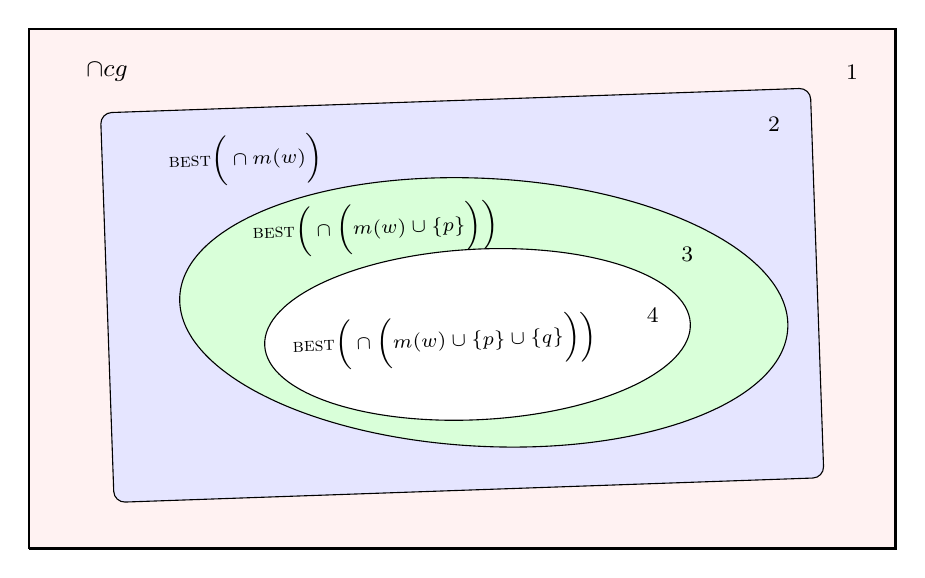
\begin{tikzpicture}[scale=2.2]
		\draw[line width=1pt,fill=red!5] (0,0) -- (5,0) -- (5,3) -- (0,3) -- (0,0);
		\node[align=center] at (.45,2.75) {\small $\cap cg$};
		\node[align=center] at (4.75,2.75) {\circled{\footnotesize 1}};
		%\draw[->] (5,2.35) -- node[above] {\footnotesize 1} (4.55,2.2) ;
		
		\draw[rotate=2,rounded corners,fill=blue!10] (.5,.25) rectangle (4.6,2.5);
		\node[align=center, rotate=2] at (1.25,2.25) {\scriptsize $\pmb{\textsc{best}\Big(\cap m(w)\Big)}$};
		\node[align=center] at (4.30,2.45) {\circled{\footnotesize 2}};
		%\draw[->] (4.55,2.15) .. controls (3.9,2.4) and (3.5,2.4) ..  node[above] {\footnotesize 2} (3.6,2);
		
		\draw[rotate=-3, fill=green!15] (2.55,1.5) ellipse [x radius=50pt, y radius=22pt]; %[postaction={decoration={text along path,		text={${best(\cap(m(w))}${}}}, decorate}] ;
		\node[align=center, rotate=2] at (2,1.85) {{\scriptsize $\textsc{best}\Big(\cap\big(m(w)\cup \{\pmb{p}\}\big)\Big)$}};
		\node[align=center] at (3.8,1.7) {\circled{\footnotesize 3}};
		%\draw[->] (3.6,1.925) .. controls (4,1.45) and (3.95,1.5)  .. node[above] {\footnotesize 3} (3.8,1.4) ; 
		
		\draw[rotate=3,fill=white] (2.65,1.1) ellipse [x radius=35pt, y radius=14pt];
		\node[align=center, rotate=2] at (2.4,1.2) {{\scriptsize $\textsc{best}\Big(\cap\big( m(w)\cup \{p\} \cup \{\pmb{q}\}\big)\Big)$}};
		\node[align=center] at (3.6,1.35) {\circled{\footnotesize 4}};
		
	\end{tikzpicture}
\end{figure}



We propose that the antecedent proposition to \textit{otherwise} --- namely, that set of worlds whose complement the consequent of \textit{otherwise} applies in, $K_{i_{\text{sub}}}$ --- can be any one of these updates in Figure 1. We spell out the resulting denotations of the three readings of the \textit{Red Light} examples in (\nextx), where $\overline{X}$ denotes the complement of the set $X$. 

\pex  \emph{Accommodated antecedent sets available in the \emph{Red Light} sentences:}
\a  \textit{If the light is red, (you) stop.} \hfill \textit{\small The pronounced antecedent}\\
(i.e. in those worlds $w'$ in which the road rules are followed and the light is red, you stop)
$$ \{ w'\in\underset{deo(w)}{\textsc{best}}(\cap\underset{\textsc{circ}}{m(w)})\mid \textsc{red.light}(w')\to\textsc{stop}(w')\} $$
%
\a  \textit{...otherwise there'd be chaos on the roads.} \hfill $=$\ref{redlightR-new-reading}\\
(i.e. in those worlds $ w_1 $ where the road rules aren't followed)\\[6pt]
\- \hfill $\{w_1\mid w_1\in\overline{\underset{deo(w)}{\textsc{best}}\big(\cap\underset{\textsc{circ}}{m(w)}\big)}\}$ 
\hfill $= \circled{1} - \circled{2} $ \\[6pt]
%
\a  \textit{...otherwise you can continue.} \hfill =\ref{redlighta-rpt0}\\
(i.e. in those worlds $ w_2 $ where the road rules are followed, but the light isn't red)\\[6pt]
\- \hfill $\{w_2\mid w_2\in\underset{deo(w)}{\textsc{best}}\Big(\cap\big(\underset{\textsc{circ}}{m(w)}\cup \overline{\textsc{red.light}}\big)\Big)\} $ \hfill $= \circled{2} - \circled{3} $ \\[6pt]
%
\a  \textit{...otherwise you'll get a ticket.} \hfill =\ref{redlightb-rpt0}\\
(i.e. in those worlds $ w_3 $ where the road rules are followed and the light is red, but you don't stop)\\[6pt]
\- \hfill $\{w_3\mid w_3\in\underset{deo(w)}{\textsc{best}}\Big(\cap\big(\underset{\textsc{circ}}{m(w)}\cup\textsc{red.light}\cup\overline{\textsc{stop}}\big)\Big)\} $ \hfill $= \circled{3} - \circled{4} $\xe


The three denotations in (b--d) correspond to the three DRSs that are modally subordinate to $K_i$, which we have argued represent the set of possible accommodated antecedents in the \textit{Red Light} examples: 

\pex  \emph{\textsc{Drs}s subordinate to $ K_i $ which can serve as the accommodated antecedent $ (K_{i_{\textup{sub}}}) $ to \emph{otherwise}:}
\a  \textbf{The modal base ($K_{m}$)}:\\ \hspace{2.5em} Road rules are followed
\a  \textbf{The conditional antecedent ($K_{m^+}$)}:\\\hspace{2.7em} Road rules are followed and the light is red. 
\a  \textbf{The entire conditional ($K_i$)}:\\ If road rules are followed and the light is red, (then you) stop. \xe


To see that other choices of antecedent are unavailable, we consider next another possible variant of the \textit{Red Light} example which, all things being equal, we might have expected to be felicitous. However, example \ref{crash-bad}, adapted from \citet[76]{Kruijff-Korbayova2001}, appears to encounter interpretation problems: it is judged by speakers as either infelicitous or false.\footnote{\citeauthor{Kruijff-Korbayova2001} do not consider explicitly the infelicity of \ref{crash-bad} (although see their discussion on p. 78).}  

\pex $ ^{\#} $If the light is red, stop; \textit{otherwise} you'll get rear-ended.\label{crash-bad}\\
\phantom{If gjdisf}\textcolor{violet}{\textsc{intended} $ \approx $ If the light is \ul{not} red and you do stop...}\xe


The intended interpretation of \textit{otherwise} in \ref{crash-bad} relies on the accommodation of a set of worlds in which the addressee stops while the light is not red. Crucially, such a set is not made available by the foregoing discourse. The discourse-salient \textit{stopping worlds} are modally subordinate to (a subset of) the \textit{red light} worlds. That is, we predict that all \textit{stopping} worlds are \textit{red light} worlds in this discourse. We correctly predict then, that $\{w'\mid w'\in\textit{\textsc{stop}}\setminus\textit{\textsc{red.light}}\}$ cannot serve as an antecedent proposition to \textit{otherwise}, explaining the infelicity of \ref{crash-bad}.\footnote{Compare \ref{crash-bad} with the vastly improved \ref{crash}, where the relevant \textit{if}-clause receives focus and associates with \textit{only}.
	
	\pex \label{crash} (Only) if the light is RED, stop; \textit{otherwise} you'll get rear-ended.\xe
	
	The felicity of \ref{crash} follows naturally from a standard semantics for \textit{only}, where \textit{only} is taken to assert the negation of alternatives to its prejacent \citep[see][99]{Horn1969}. As shown by \citet{McCawley1974, Barker1993} and \citet{VonFintel1994, VonFintel1997}, the truth-conditional content of \textit{only if} can be derived compositionally (\textit{i.e.} as a function of the standard semantics of \textit{only} and \textit{if}), where the assertive content of $ q, $\textit{ only if} $ p $ is modeled as $ \neg p(w) \to \neg q(w)$ (that is, $ q $ holds in no worlds other than those in which $ p $ does). 
	
	\pex \textit{Presuppositional and assertive components of \ref{crash}:}\\
	Only if the light is RED, stop; \textit{otherwise} you'll get rear-ended.\\ 
	\uline{Presupposes}: If the light is red, you stop.\\
	\uline{Asserts}: If the light is \{yellow | green\}, you don't stop. If you do stop, you get rear-ended. \xe
	
}

Finally, consider an example with several conjoined clauses. In (\nextx), either all three conjoined clauses or the \textit{final} conjunct can be  accommodated as an antecedent proposition to \textit{otherwise}. The other conjuncts are not accessible antecedents for \textit{otherwise} in this context on their own. Again, this is precisely what is predicted from a modal subordination account.


\pex  You should have a snack, chill out for a bit, and then you should go to the gym, \textit{otherwise} you'll feel bad later on.\xe


In sum, we have shown that each of the three \textit{Red Light} sentences investigated here can be represented by the \textit{otherwise} condition (i.e. $ K_i\ominus K_j $) given in \ref{otherwise-complex} (formalized in DRL terms in the appendix as \ref{satcon}). %Their truth relative to a model is verified iff there is some way of embedding them \citep[\textit{cf}][693]{Roberts1989}.  
As discussed at length, the choice of antecedent for \textit{otherwise} varies between the examples, and cannot be determined from the preceding syntax alone. Instead, we have argued that the proposition which is accommodated as the antecedent to \textit{otherwise} is selected from {a set of propositions made salient by the pronounced antecedent $ K_i $: those that are accessible from $ K_i $ and which monotonically restrict the context set/the domain of a modal operator.}\footnote{\label{biscuit}An anonymous reviewer queries the applicability of this proposal to relevance/biscuit-type conditionals such as (a) below. We believe that the analysis defended here can be reconciled with previous accounts of biscuit conditionals (\citealp[e.g.][]{Siegel2006, Franke2007} a.o.). Very roughly, a sentence of the type (a) below can be paraphrased as (b) --- that is, the negation of the entire biscuit conditional furnishes an antecedent to \textit{otherwise}.
	\pex\a \textit{If you're hungry, there's pizza in the fridge. \emph{Otherwise}, there are biscuits on the sideboard.}
	\a (You are hungry $ \wedge \neg$ \textsc{relevant} (Pizza in fridge)) $ \Rightarrow $ \textsc{relevant}(biscuits on sideboard)\xe
}

% biscuit fn

%
%The prejacent to \textit{otherwise} $ K_j $, is modally subordinate on a set of propositions which that are made salient in a given discourse context --- those which montonically restrict the context set. 
%
%In the modalized examples analyzed here, we saw that this was a contextually determined modal base $\boldsymbol{ K_m} $, that modal base restricted by a conditional antecedent $ K_m\Cap K_a=\boldsymbol{K_{m^+}} $ and the entire conditional $K_{m^+}\Rightarrow K_c=\boldsymbol{K_i} $. Shown in \ref{subord-tree}. This is the set of DRSes accessible from $ K_i $ that aren't modally subordinate to other propositions (i.e. that have no sister on their left).\mcom{this gen isn't quite right cos Km$ \leq $Km+}
%
%Different options are available, which, we have proposed, amount to the set of modally subordinate propositions to the pronounced antecedent to \textit{otherwise}. 

The consequent clause plays a crucial role in the reasoning about which proposition among this set represents the set of worlds under consideration in the evaluation of an \textit{otherwise}-sentence. We discuss this reasoning in detail in section \ref{sec:qud}. %\mcom{still a bit of an issue with the generalisation: something like: ``chosen out of a set of accessible propositions that restrict the domain of a modal operator??'' \textcolor{red}{tweaked, take a look}\textcolor{forest}{ slightly more tweaked, take a re-look}}


%\clearpage
\subsection{\emph{Otherwise} as a discourse anaphor}\label{sec:qud}

As the preceding sections make clear, there is often more than one possible choice for the antecedent proposition of \textit{otherwise}. How is this antecedent chosen, then? We propose that the antecedent proposition which \textit{otherwise} operates on is calculated pragmatically from the prior discourse and the nature of the consequent clause.\footnote{This claim bears some similarity to the notion of an ``anaphorically-derived contextual parameter'' that features in the analysis of \citet[14]{Webber2001}.}$ ^, $\footnote{Relatedly, \citet{Corblin2002} notes the possibility of \textit{negative accommodation} without \textit{otherwise} in \textit{I didn't buy the car. I wouldn't have known where to put it (otherwise)} and \textit{I should have accepted. I wouldn't have been fired.} (our translations: 256, 258).}

By deploying the information structure notions developed in \citet{Carlson1983} and \citeauthor{Roberts1996} (\citeyear{Roberts1996}/\citeyear{Roberts2012}), we can conceptualize of \textit{otherwise} as representing a \textsc{discourse move} (in effect, a stage in a given discourse), which adds to the \textsc{Question under Discussion} in a given discourse context $ \mathcal D $.

\pex  \textit{Two useful definitions:}
\a  The \textbf{common ground} is a set of mutually assumed background information. The $cg$ is often modeled as a set of propositions, i.e.  a set of sets of possible worlds (e.g. \citealt{Stalnaker1979} \textit{et seq.}). \label{common-ground}
\a  The \textbf{QuD} is a partially structured set of questions which discourse participants are mutually committed to resolving at a given point in time. It is often modeled as a stack, consisting of ordered subsets of accepted question moves, the answers to which are not entailed by the $cg$ (\textit{i.e.}, a set of ``open'' questions in the discourse at a given time.) \xe

With these concepts, we have a means of representing the `flow' of information and changes in the interlocutors' information states over time. We take a sentence of the form $ p $ \textit{otherwise} $ q $ to consist of (at least) three discourse moves. We propose that \textit{otherwise} represents a discourse ``setup'' move with the effect of adding to the \textsc{QuD}. 

\pex  \emph{Proposal: the pragmatics of \emph{otherwise}}\\
\textit{Otherwise} represents a discourse ``setup'' move with the effect of adding to the \textsc{QuD} stack a question about the \textsc{complement} of a set of worlds calculated on the basis of the utterance preceding \textit{otherwise}.\xe

The importance of this pragmatic aspect of our analysis is illustrated for example (\nextx) below. 


\pex  \label{eat} [\textit{You must eat}]$_{m_i}$, \textbf{otherwise}$ _{m_j} $ [\textit{you won't grow!}]$_{m_k}$\xe


\begin{itemize}%[label={\textit m}{\tiny\arabic*}.]
	\item[ {\makebox[2.5em][r]{$ m_i $}} ] This is the pronounced antecedent. It represents a modalized assertion: the addressee eats in all worlds in some unspecified conversational background (here, likely some teleological ordering source containing the subject's goals or some set of nutritional standards --- e.g. $ \underset{\textit{tel(w)}}{\textsc{best}}\big(\cap\underset{\textsc{circ}}{m(w)}\big)  $
	$$\forall w'\big[w'\in\underset{\textit{tel(w)}}{\textsc{best}}\big(\cap\underset{\textsc{circ}}{m(w)}\big) \to \textsc{eat}(\textit{Addressee})(w')\big]$$
	\item[ {  \makebox[2.5em][r]{$ m_j $}} ]\textit{otherwise} represents an instruction to consider the \textsc{complement} of some set of worlds accessible from the pronounced antecedent. This can be thought of as signaling the addition of a question to the \textsc{QuD} stack of the form: $$
	\lambda p\,.\,\text{ what if we are in some } w\in\overline{\boldsymbol p}\text{ ?}$$
	
	(As above, the $ \overline{\text{overline notation}} $ denotes a function that maps a set of worlds to its complement.) In this case, a plausible candidate is: what if we are in a world in which the addressee doesn't eat?
	
	\item[ {  \makebox[2.5em][r]{$ m_k $}} ] The consequent clause to \textit{otherwise} is interpreted as proffering a (partial) answer to the current \textsc{QuD} by asserting  that -- as far as the speaker is concerned -- the addressee won't grow in the set of worlds made available to \textit{otherwise} --- here, the complement of the set of worlds that best adhere to some set of goals/nutritional standards in $ w $.
	%todo, note that i've changed the analysis of this sentence so it conforms with the previous discussion: we can /should discuss whether or not this makes sense
	%todo -- old formalism $${\forall w^{\prime\prime}\!\big[w''\!\in\textbf{\textsc{compl}}\big(\textsc{eat(\textit{Addressee})\big)}\to\neg\textsc{grow}(Addressee)(w^{\prime\prime})}\big]$$
	$$\forall w^{\prime\prime}\big[w''\!\in\underset{o(w)}{\textsc{best}}\big(\cap \underset{\textsc{circ}}{m(w)}\cup\overline{\textsc{eat}(w^{\prime\prime})}\big)\;\square\;\neg\textsc{grow}(w^{\prime\prime})\big]$$
	
	%		Pragmatically, as Inkova-Manzotti observes (2001), the \textit{otherwise} clause canonically (\textit{``l'emploi prototypique''}) appears to encode a situation that is undesirable for the interlocutor. Indeed, the retrieval of a bouletically ordered conversational background to the modal in $p$ appears to be informed by the probable implication of the undesirability of the prejacent.
\end{itemize}

As we know, the process of establishing the context set for a given \textit{otherwise} sentence is underdetermined by the syntax of the sentence.\footnote{In our example in (\lastx), an alternative \textsc{QuD} raised by \textit{otherwise} could be ``what if we are in a world in which the addressee doesn't have to eat?'' However, this potential question can be dismissed on the grounds that the consequent ``you won't grow'' isn't a plausible answer to this question. We discuss this issue at length next.} In the context of the \textit{Red Light} sentences, the discourse moves $ m_i,m_j,m_k $ in the pronounced antecedent are identical. However, the consequent clauses of \ref{redpuzzle-0}, \ref{red-puzzlea} and \ref{red-puzzleb} contribute the moves $m_a$, $m_b$, and $m_c$, respectively. The fact that these moves are different suggests that a different question move can be raised (added to the \textsc{QuD)} by \textit{otherwise} in each case.

\pex \textit{Three different discourse moves based on the same antecedent:}\label{red-puzzle} 
\a \label{redpuzzle-0} [\textit{If the light is red},]$_{m_i}$[ \textit{stop};]$_{m_{j}}$ \textit{otherwise}$ _{m_k} $ [\textit{there will be chaos.}]$_{m_{a}}$ 
\a  \label{red-puzzlea}[\textit{If the light is red},]$_{m_i}$[ \textit{stop};]$_{m_{j}}$ \textit{otherwise}$ _{m_k} $ [\textit{keep going.}]$_{m_{b}}$ 
\a  \label{red-puzzleb}[\textit{If the light is red},]$_{m_i}$[ \textit{stop};]$_{m_{j}}$ \textit{otherwise}$ _{m_k} $ [\textit{you'll get a ticket.}]$_{m_{c}}$ \xe

We provide an Information-Structure based analysis for this state of affairs. We spell this out in \ref{is-puzzle}--\ref{is-jeopardy} below:  

\pex \textbf{An information-structural approach to the \textit{Red Light }puzzle}\label{is-puzzle}
\begin{enumerate}
	\item[ {  \makebox[2em][l]{$ m_i $}} ] The \textit{if}-antecedent temporarily constrains the context set \citep[687]{Roberts1989}. This might be thought of as adding a question to the \textsc{QuD} stack of the form: $$ \text{what if we are in} \{w'\mid w'\in\underset{o(w)}{\textsc{best}}\Big(\bigcap\big(m(w)\cup\textsc{red.light}\big)\Big)\}? $$
	%	
	\item[ {  \makebox[2em][l]{$ m_j $}} ] Imperative \textit{stop} represents an answer to $ \textsc{QuD}(m_i)$. As with the antecedent in \ref{eat}, we treat it as a modalized proposition (again with some conversational background \textit{f})\footnote{See \citet{Portner2007} a.o.\ for a modal treatment of imperative sentences.} which further restricts the domain established by $ m_i $.\\
	$$\forall w''\big[\hspace{3pt} w''\in\underset{deo(w)}{\textsc{best}}\big(\bigcap\underset{\textsc{circ}}{m(w)}\cup\textsc{red.light}\big)\to w''\in\textsc{stop}(\textit{Addressee})\big]$$
\end{enumerate}\xe
%todo for completeness the modal base should be here (and probably in m_i also, but maybe it's just all a bit much.)


Per our proposal, \textit{otherwise} marks the addition of a question to the \textsc{QuD} stack which considers what would happen if we were in the \textit{complement} to a proposition accessible from the pronounced antecedent: 

\pex  \label{is-otherwise} \emph{The \emph{otherwise} discourse move:}
\begin{itemize}
	\item [ { \makebox[2em][l]{$ m_k $}} ] \textit{Otherwise} represents an instruction to consider the \textbf{complement} of some set of worlds accessible from the pronounced antecedent. 
	$$\lambda p\,.\,\text{what if we are in some }w\in\overline{\boldsymbol p}\text{ ?}$$
\end{itemize}\xe

$m_i$ and $m_j$ have both introduced sets of worlds constraining the context set: each of these sets of worlds represents a candidate that \textit{otherwise} can be anaphoric upon. Moreover, as we have seen in previous sections, the \textit{modal base} of a modalized proposition is also an accessible set of worlds that can be questioned.
The Addressee is thus required to \textit{infer} which of these multiple restrictions \textit{otherwise} is anaphoric upon (\textit{i.e.}, its antecedent), based on the content of the consequent. We dub this the \textit{jeopardy! effect}: the addressee is provided with the consequent (=the answer) and must compute (\textit{sc.} accommodate) the correct antecedent (=question) based on it:\footnote{This bears some similarity to the account of discourse-anaphoric uses of \textit{then} laid out in \citealt{Biezma2014}: ``\textit{then} is a discourse marker that signals that the utterance of the embedded clause is in some sense motivated by [and therefore is \textbf{anaphoric upon}] the preceding discourse move'' (380, 383).} 

\pex \textit{The \textsc{Jeopardy!} effect} \label{is-jeopardy}
\begin{itemize}
	\item [ { \makebox[2em][l]{$ m_a $}} ] \textit{there will be chaos} is interpreted as an answer to \textit{what if we are in} \textbf{the complement} of the modal base? (those worlds in which the road rules of in $ w $ don't hold) %\\[.3em]Here the propositional variable is saturated by a partition evoked in $ m_i $.%\\[.15em]
	$$ \forall w''\big[w''\in\overline{\textsc{best}(\cap m(w)})\,\square\, \textsc{keep.going}(w'')\big] $$ 
	%  
	\item [ { \makebox[2em][l]{$ m_b $}} ] \textit{keep going} is interpreted as an answer to \textit{what if we are in} \textbf{the complement} of \textsc{red.light} (relative to the modal base)?
	$$ \forall w''\big[w''\in\textsc{best}(\cap(m(w)\cup\overline{\textsc{red.light}}))\,\square\, \textsc{keep.going}(w'')\big] $$
	%
	\item [ { \makebox[2em][l]{$ m_c $}} ] \textit{get a ticket} is interpreted as an answer to \textit{what if we are in}\\ ${\textsc{red.light} \setminus\textsc{stop}}$? (more accurately, the complement of \textsc{stop} \textit{relative} to the conditional modal base $ m^+(w) $) %\\[.3em]Here a sub-partition (within the set of ``red light worlds'') evoked in $ m_j$ saturates the propositional variable (the mechanisms predicting the availablity of these sets were spelled out in \S\ref{sec:illustration}).
	\begin{flalign*}
		\forall w''\big[w''\in\textsc{best}(\cap(m(w)\cup\textsc{red.light}\cup\overline{\textsc{stop}}))\,\square\, \textsc{get.ticket}(w'')\big] 
		%=\forall w''\big[w''\in\{\textsc{red.light}  \cap  \textbf{compl}(\textsc{stop})\}\to \textsc{get.ticket}(w'')\big] 
	\end{flalign*} 
\end{itemize}\xe
%\mcom{\textcolor{red}{$m^+$ makes an appearance again, but only here and not in the other readings. Intended? choose and stick with one notation.}} 

\noindent Our claim, then, is that computing the antecedent of \textit{otherwise} is a pragmatic process, subject to reasoning by the addressee and depending on the given context in which the sentence is uttered.\footnote{This makes predictions for online sentence processing --- for example, that a given reading could be primed or ruled out by supporting contexts. We leave this for future work.} This follows from the pragmatic stipulation that, in a discourse, assertions represent `at least partial answers [...] to the question under discussion at the time of utterance' (\citealp[20--21]{Roberts2012}, see also \citealp{Roberts2004} on the ``domain goals'' of discourse participants and how these can direct participants' ``strategies of inquiry.'')\footnote{In fact, this effectively serves as a reformulation and elaboration of Grice's maxim of Relation, adapted for an information-structural framework.} Broadly, the discourse contribution of \textit{otherwise} can be understood as representing a ``set-up move'': it signals to the addressee that its consequent is to be understood as a modal claim, relativized to the complement of a set of worlds accessible from the pronounced antecedent. 



\section{\textsc{Non-emptiness} and possibility modals}
\label{sec:predictions}

%todo: note also discussions (summ in HAc 11) that epistemics make no truth conditional contribution
Given that, on the analysis presented in the foregoing section, \textit{otherwise} requires reference to a set of ``eliminated worlds''---the complement of some set of worlds introduced by the antecedent clause---it follows that a sentence of the form $ p \textit{ otherwise } q$ will be uninterpretable in discourses in which \textbf{no} worlds have been eliminated (i.e. where $ \overline{p'}=\varnothing $). This principle is formulated in \ref{felcon}, and reflects the \textit{non-emptiness} requirement we observed in section \ref{sec:non-emptiness}.

\pex \label{felcon}\textit{\textsc{Exclusion}: a felicity condition for \emph{otherwise}}\\
The interpretation of \textit{otherwise $ \alpha $} depends on the retrieval of some discourse move whose function was to eliminate a (nonempty) set of worlds $ \beta $ from consideration (i.e., from the context set).\\$ \textit{Otherwise}\,\alpha $ predicates $ \alpha $ of $ \overline\beta $.\xe

In this section we show two consequences of this criterion for the interpretation of \textit{otherwise} in modalized sentences. 


\subsection{Unambiguous scope} \label{sec:scope}

A sentence like \textit{Sam may not be a doctor} is ambiguous between circumstantial and epistemic readings for the modal. With this in mind, observe the contrast between \ref{sam-circ}/\ref{sam-nec} and \ref{sam-pos} below, which we argue further demonstrates the interpretive constraints that \textit{otherwise} is subject to --- namely, that it must be able to refer to a non-empty complement set of worlds, computed on the basis of its antecedent and other components of the context. To illustrate this, consider the three contexts provided for these examples. These are designed to support a circumstantial possibility reading \ref{sam-circ}, and epistemic necessity and possibility readings \ref{sam-nec}--\ref{sam-pos}, in the context of an \textit{otherwise} statement:

\pex  \textsc{context.} Sam got horrible grades in school and is very clumsy\label{sam-circ}
\a   She may not be a doctor, \textit{otherwise}...\hfill$ \neg\gg\lozenge_\text{circ} $
\a  \makebox[0.45\textwidth][l]{\textcolor{violet}{$ \approx $ If she were (to become) a doctor...}} ...she might kill someone.\xe


\pex  \textsc{context.} Sam works in a hospital and wears a white coat; I'm unsure exactly what it is that she does, but upon soliciting her opinion on my shoulder pain, she shrugs and walks away.\label{sam-nec}
\a   She must not be a doctor, \textit{otherwise}...\hfill $ \square_\text{epist}\gg\neg $
\a  \textcolor{violet}{$ \approx $ If she \uline{were} a doctor...} \,\,\,\,...she'd know what to do about my pain.\xe

\pex  \textsc{context.} Sam works in a hospital and wears a white coat; I'm unsure what exactly it is that she does.\label{sam-pos}
\a   She may not be a doctor, \textit{otherwise}...\hfill $ 	*\lozenge_\text{epist}\gg\neg $
\a  {\textcolor{violet}{\textsc{intended $ \approx $} If she \uline{is} a doctor...}} \hspace{2em}$ ^{??}$...she's probably a surgeon.
\xe

Observe that, while examples \ref{sam-circ} and \ref{sam-nec} are acceptable, \ref{sam-pos} is not. A crucial difference between the circumstantial \ref{sam-circ} and epistemic \ref{sam-pos} readings of the antecedent is the scope relation between the possibility modal and the negative operator. Just as for example \ref{school} discussed in section \ref{sec:non-emptiness} above, \textit{otherwise} is only licit if it can predicate into a non-empty set of worlds. In the $ \neg\gg\lozenge $ case (as in the $ \square\gg\neg $ case) we can successfully achieve this result. But in the  $ \lozenge\gg\neg $ case, where there is no set of worlds eliminated, \textit{otherwise} is unavailable. That is, whether or not Sam is a doctor \ul{is not determined} by the antecedent clause in \ref{sam-pos}. As a result of the infelicity of \textit{otherwise} in these $ \lozenge\gg\neg $ contexts (owing to the \textsc{exclusion} criterion), epistemic readings of \textit{may} are ruled out; only the (narrow scoping) circumstantial reading---as in \ref{sam-circ}---is available. Finally, example \ref{sam-nec} as a control, to show us that, in general, an epistemic modal is able to scope above negation and hence that cannot be the source of the infelicity of \ref{sam-pos}.

%Given \textit{otherwise}'s observed infelicity with possibility readings of \textit{may}, the epistemic reading is ruled out, leaving only a circumstantial one available.%Here, this result correlates with the possible reading of \textit{may}, ruling out the epistemic reading and leaving only the circumstantial one available.


\subsection{Epistemic strengthening} \label{sec:epistemic}


A second, related result concerns so-called `weak necessity' readings of possibility modals \citep{Rubinstein2012, VonFintel2008}.

The modals \textit{ought} and \textit{should} have been described as encoding ``weak'' necessity, distinguishing them from other modal necessity expressions (e.g. \textit{have to} and \textit{must}.) Two examples demonstrating the relation between weak and strong necessities from \citet[117]{VonFintel2008} are provided below.

\pex  \textit{Weak and strong necessity:}
\a  You \textit{ought to} do the dishes but you don't \textit{have to}.
\a  \hspace{-.35em}$ ^{\#} $You \textit{must} do the dishes but you don't \textit{have to}\xe
\pex  \a You \textit{ought to} wash your hands -- in fact, you \textit{have to}.
\a  \hspace{-.35em}$ ^{?} $You \textit{have to} wash your hands -- in fact, you \textit{ought to}.\xe
%	\textcolor{red}{JP: I think b might actually be okay with a reading like, ``scrap that, it's not the case that I actually \textit{need to}, but i \textit{should}. Is this a problem?}\xe

Additionally, as with other modals, \textit{ought} appears to admit of ambiguity between epistemic and circumstantial (e.g. deontic) readings, as shown in \ref{ought}.\footnote{Cf. \citet{Yalcin2016} for a dissenting view, namely the claim that epistemic modality cannot be `sensitive to normality orderings' (239) and that \textit{ought} and \textit{should} don't actually admit of a true epistemic reading.}

\pex \label{ought} \textit{Weak necessity and modal flavors:}\\
Morris \textit{ought to} be in his office.\hfill\citep[116]{VonFintel2008}\xe


In view of the co-occurence constraints on epistemic possibility modals with \textit{otherwise}, compare the two sentences (both judged as acceptable) in \ref{sick}: %Example \ref{sick-might} shows that the possibility modal \textit{might} can likewise receive a strengthened interpretation in the context of \textit{otherwise}: 


\pex \label{sick} \textit{A felicitous epistemic possibility modal with \emph{otherwise}:}
\a  She \textit{must} be sick, otherwise she'd be here. \label{sick-must}%\\
%			\hspace*{1em}$=\forall w'[w'\in\textsc{best}(\cap( \underset{\textsc{epist}}{m(w)}\cup\overline{\textsc{sick}})\to w'\in \textsc{here}]$\\
%			\hspace*{1em}$ \overline\alpha=\{w\in f_{\text{epist}}\mid \text{She is not sick in }w\} $
\a  She \textit{might} be sick, otherwise she'd be here. \label{sick-might}\xe

%\begin{figure}[h]\label{cg-updates-fig}\caption{Updates to the common ground as monotonic restrictions on the set of worlds under consideration. \textit{Otherwise} can ``target'' the complement set of one of these restrictions (i.e. any of the three disjoint, shaded regions).}\centering
%	\begin{tikzpicture}[scale=1.9]
%		\draw[line width=1pt,fill=red!5] (0,0) -- (5,0) -- (5,3) -- (0,3) -- (0,0);
%		\node[align=center] at (.45,2.75) {\small $\cap cg$};
%		\node[align=center] at (4.75,2.75) {\circled{\footnotesize 1}};
%		%\draw[->] (5,2.35) -- node[above] {\footnotesize 1} (4.55,2.2) ;
%		
%		\draw[rotate=2,rounded corners,fill=blue!10] (.5,.25) rectangle (4.6,2.5);
%		\node[align=center, rotate=2] at (1.25,2.25) {\scriptsize $\pmb{\textsc{best}\Big(\cap\underset{\textsc{epist}}{m(w)}\Big)}$};
%		\node[align=center] at (4.30,2.45) {\circled{\footnotesize 2}};
%		%\draw[->] (4.55,2.15) .. controls (3.9,2.4) and (3.5,2.4) ..  node[above] {\footnotesize 2} (3.6,2);
%		
%%		\draw[rotate=-3, fill=green!15] (2.525,1.5) ellipse [x radius=50pt, y radius=22pt]; %[postaction={decoration={text along path,		text={${best(\cap(m(w))}${}}}, decorate}] ;
%%		\node[align=center, rotate=2] at (2.1,1.85) {{\scriptsize $\textsc{best}\Big(\cap\big(\underset{\textsc{epist}}{m(w)}\cup \{\textsc{sick}\}\big)\Big)$}};
%%		\node[align=center] at (3.8,1.7) {\circled{\footnotesize 3}};
%		%\draw[->] (3.6,1.925) .. controls (4,1.45) and (3.95,1.5)  .. node[above] {\footnotesize 3} (3.8,1.4) ; 
%		
%%		\draw[rotate=3,fill=white] (2.65,1.1) ellipse [x radius=35pt, y radius=14pt];
%%		\node[align=center, rotate=2] at (2.4,1.2) {{\scriptsize $\textsc{best}\Big(\cap\big( m(w)\cup \{p\} \cup \{\pmb{q}\}\big)\Big)$}};
%%		\node[align=center] at (3.6,1.35) {\circled{\footnotesize 4}};
%		
%	\end{tikzpicture}
%\end{figure}

The domain restriction in \ref{sick-must} proceeds similarly to the examples described in the previous section. %(that is, the prejacent to \textit{otherwise} is predicated of those worlds $ \{w'\mid\textsc{best}(\cap(m(w)\cup\overline{\textsc{sick}}))\}$). The first clause of \ref{sick-might}, uttered in isolation, asserts the existence of epistemically-accessible worlds in which the subject is sick (i.e. $ \exists w'\in \cap f_\text{epist}.\text{ She is sick in } w'$). 
That is, the antecedent has eliminated \textsc{non-sick} worlds from the epistemic context set. The \textit{otherwise} clause is then predicated of these \textsc{non-sick} worlds that best conform to the speaker's knowledge state.

However, example \ref{sick-might} presents a puzzle: the use of a possibility modal suggests that as far as the speaker is concerned, the subject may or may not be sick. That is, \textsc{non-sick} worlds are \textit{not} eliminated from the context set. 
%an epistemic possibility reading %\footnote{That is where the entire antecedent $ \lozenge(\textit{she \textsc{be} sick)}$ is accommodated and its negation restricts the domain of \textit{otherwise.}}
% is not available because no possible worlds have been excluded from the context set (that is, as far as the speaker is concerned, the world may or may not be sick).
Consequently, the felicity condition for \textit{otherwise} as laid out in \ref{felcon} is not met: unlike in \ref{sick-must}, the \textsc{non-sick} worlds cannot be accommodated as a restrictor to \textit{otherwise}. We would therefore predict \ref{sick-might} to be ungrammatical, contrary to the facts.

This problem is repaired here by \textit{strengthening} the meaning of \textit{might}, so that it is interpreted as excluding a set of possible worlds (that is, requiring that it function as a universal quantifier: a hallmark of necessity modals). While the intended interpretation of \ref{sick-might} is weaker than that of its counterpart in \ref{sick-must}, it can still be understood as quantifying \ul{universally} over possible worlds, albeit over a more restricted set. 
Following \citet[116, fn. 11]{VonFintel2008}, `while strong necessity modals say the prejacent is true in all of the favored worlds, weak necessity says that it is true in all the very best (by some additional measure) among the favored worlds.' With respect to the epistemic domain specifically, the difference could be understood as the difference between relativizing the prejacent to ``hard and fast evidence'' and ``unreliable assumptions about the normal course of events.''\footnote{\Citet{VonFintel2008} and \citet{Rubinstein2012} model weak necessity by appealing to at least one additional (``secondary'') ordering source which ``refines the ranking of worlds'' --- weak necessity modals predicate their prejacent of ``all the very best'' (according to some set of criteria) of the worlds in the modal base that are already ranked best.  In the current case, the secondary ordering source might be described as some species of \textit{stereotypical} conversational background $ o_2 $ that includes propositions about the speaker's perception of the subject's disposition/general conduct. Adopting this analysis, the accommodated antecedent for \ref{sick-might} is:
	
	\pex  $\overline{\alpha}=\Big\{w'\mid w'\in\underset{o_2(w)}{\textsc{best}}\Big(\underset{o_1(w)}{\textsc{best}}\big(\cap (\underset{\textsc{epist}}{m(w)}\cup\overline{\textsc{sick}})\big)\Big)\Big\} $
	%\b. $ \overline\alpha=\{w\in\textsc{best}_{g_{st}}(f_{\text{epist}})\mid \text{She is not sick in }w\} $\xe
	
	\xe} %fn 
Consequently, we propose the paraphrases below:

\pex  \textit{With \emph{otherwise} the possibility modal is strengthened to weak necessity:}
\a  She \textit{must} be sick, otherwise she'd be here.\\
$\approx$ \textit{In all worlds consistent with what I know,}\\ \hspace*{0.7em} if she is not sick, she'd be here. 
\a  She \textit{might} be sick, otherwise she'd be here.\\
$\approx$ \textit{In all worlds consistent with my perception of her general behavior},\\ \hspace*{0.7em} if she is not sick, she'd be here.\xe

The finding that \textit{might/may} --- generally understood as encoding modal possibility --- are in these contexts apparently encoding weak necessity suggests that the felicity conditions of \textit{otherwise} \textit{coerce} a non-canonical interpretation of these modals.\footnote{We leave a proper analysis of the mechanism by which this ``strengthening'' occurs to future research, although, %by hypothesis, a universal-type reading of \textit{might} is coerced here by the semantics of \textit{otherwise}. 
	given that \textit{might} is a ``weak'' scalemate of \textit{must}, it follows that---in contexts which require a necessity interpretation---the interpretation of \textit{might} would be ``weak'' relative to \textit{must}.} This result follows from our proposal in section \ref{sec:proposal} (and the exclusion criterion in \ref{felcon}), that some non-empty set of worlds must be available for \textit{otherwise} to predicate of. %In this section we observed two ways in which this requirement is enforced: through the elimination of an otherwise available scope reading in section \ref{sec:scope}, and through epistemic strengthening in section \ref{sec:epistemic}.

%
%todo can't find a place for this, and there's not much of an analysis. Leaving out.  
%
%The value of building an accessibility relation into a proper treatment of \textit{otherwise} is shown by the minimal pair in \ref{pierre} below. \citet[125$ ^\tau $]{Inkova-Manzotti2002} notes the where epistemic adverbials (e.g. \textit{probably}) favour what she refers to as a ``justificatory'' reading, this reading is blocked in contexts that `presuppose the truth of [their prejacent]' (e.g. (un)fortunately) 
%
%\pex \label{pierre}\a.\label{pierre-epist} Peter's probably left. \textit{Otherwise} his car would be in the lot.\\
%\b.\label{pierre-fact} $ ^\# $Peter's left, thankfully. \textit{Otherwise} his car would be in the lot.\\\xe
%
%In each example above, while \textit{otherwise} retrieves a different the same antecedent --- $ \lambda w.\text{Peter has left in }w$ ---, however the adverbial in the first sentence influences the ``modal flavour'' of \textit{otherwise}. The analysis defended here captures this distinction by requiring that \textit{otherwise} contextually retrieve a premise set.
%
% In \ref{pierre-epist}, the epistemic adverb \textit{probably} leads to the likely retrieval of an epistemic modal base whereas in \ref{pierre-fact} the factive adverb \textit{thankfully} effects the retrieval of a metaphysical one, realistically ordered.
%
%



\section{Intra-sentential \textit{otherwise} and complement anaphora}
\label{sec:bonus}
%{\color{gray}\mcom{Unsure if this recap is necessary here, I'm not sure where it came from actually...}So far, we have proposed an analysis of \textit{otherwise} as a discourse-sensitive conditional: \textit{otherwise} adds to the QuD a question of the form: \textit{what if the antecedent doesn't hold?}, where the nature of the antecedent must be computed from the preceding discourse context. We showed that this pragmatic account is able to naturally explain cases of ambiguity in the choice of antecedent, as well as how it is constrained. In particular, the notion of modal subordination from \citealt{Roberts1989} \textit{et seq} played a crucial role in this regard. We claim that the syntax on its own cannot on its own furnish the right antecedent for \textit{otherwise} in all the cases we considered.}
%
%

So far, the data we have focused on in this paper have comprised uses of \textit{otherwise} that appear to signal a relation between clauses. We have claimed that, in these cases, \textit{otherwise} adds a question of the form \textit{what if the antecedent proposition doesn't hold?} to the \textsc{QuD} stack. Nevertheless, as shown in section \ref{intro}, intra-sentential uses of \textit{otherwise} --- namely, those which coordinate smaller structures --- are also available. In this section, we briefly show how our analysis might be extended to account for such uses. We then relate our analysis to the phenomenon of \textit{complement anaphora}, which has also benefited from an analysis within a dynamic semantic framework.

%\pex  \label{intrasent}
%\a. The income they earn from it is likely to be the only source of cash to supplement their \textit{otherwise} subsistence economy.\hfill(\textsc{oed})
%\b. \label{amelia} Amelia behaved well \textit{otherwise}. \hfill (\citealt{Flament-Boistrancourt2011})
%\c. \label{bigissue} Every person selling ``The Big Issue'' might \textit{otherwise} be asking for spare change. \hfill \citep{Webber2001}\xe




\subsection{\textit{Otherwise} with donkey anaphors} 
\label{sec:etype}


A key advantage of DRT is in providing an analysis of so-called Donkey Sentences, such as in (\nextx): 

\pex  \textit{Donkey anaphora:}
\a  If a woman is rich, she owns a donkey. 
\a  If a dog is hungry, Pedro might feed it.  \hfill =\ref{donkey}\xe

Such sentences were famously used as a counter-examples to Montague's formal analysis of quantification in natural language \citeyearpar{montague1973}, as they defy an analysis in first-order predicate logic.\footnote{A formula can be given, but only if the indefinite is translated using a universal quantifier --- an arguably undesirable result.} As we saw in section \ref{sec:DRT}, DRT is able to provide a natural account, treating indefinites as variables rather than existential quantifiers (see \citealt{Kamp1981}, \citealt{Heim}). This is exemplified again in (\nextx): 

\pex  \drs{~}{
	\drs{x}{woman(x)\\rich(x)\,\,}~{\Large$\Rightarrow$}\drs{y}{
		donkey(y)\\owns(x, y)}}
\xe


One payoff of the approaches espoused by these authors is the conception of universal expressions as complex conditions of the form $K_i \rightarrow K_j$, where $K_i$ and $K_j$ are sub-DRSs representing the restriction and the scope of the quantified statement, respectively \citep[693-4]{Roberts1989}. 

Appealing to these same notions, we are able to naturally account for some intra-sentential uses of \textit{otherwise}, as in (\nextx) from \citealp[7]{Webber2001}, repeated here for convenience:


%\clearpage
\pex  \label{bigissue-rpt} \textit{Intra-sentential \emph{otherwise}:}\label{intra-adv}
\a  Every person selling ``The Big Issue'' might \textit{otherwise} be asking for spare change. \trailingcitation{=(\ref{bigissue})}
%
%%Let $ S_{\langle s,\langle e,t\rangle\rangle} $ represent the property of being a seller of \textit{The Big Issue} and $ A_{\langle s,\langle e,t\rangle\rangle} $ represent the property of asking for spare change. The DRT representation in (\nextx) will then schematize the meaning of (\lastx): 
%
\a  \drs{X}{X = $\sum x$ \\ person(x)\\
	\drs{~}{sell.the.Big.Issue(x)}~{\Large$\ominus$}\drs{~}{
		{\Large$\lozenge$}\drs{~}{
			ask.for.spare.change(x)}
}}
\a  $\approx$ In all worlds in which a person $x$ isn't selling the Big Issue, it's possible that the person $x$ is asking for spare change. \xe
%
%
%\pex \label{bigissue-DRS}\begin{tikzpicture}[baseline=(current bounding box.north)]
%\draw (0.5,0) -- (8,0) -- (8,4) -- (0.5,4) -- (0.5,0);
%\draw (1,.5) -- (3.5,.5) -- (3.5,3.5) -- (1,3.5) -- (1,.5);
%%\draw[thick] (.25,.25) -- (3.75,.25) -- (3.75,3.75) -- (.25,3.75) -- (.25,.25);%%outerbox of antec
%\node[align=center] at (2.25,2) {$x$\\\\\\ $S(x)$};
%\draw (7.5,.5) -- (5,.5) -- (5,3.5) -- (7.5,3.5) -- (7.5,.5);
%\node[align=center] at (6.25,2) { $u$\\\\ $ A(u)$\\  $u=x$};		
%\node[align=center] at (4.25,2) {{\LARGE$\boldsymbol\ominus$}}; %otherwise op
%%\node[align=center] at (.625,2) {{$\boldsymbol\square$}}; %cons op
%\end{tikzpicture}\\
%	\c. $\llbracket\ref{bigissue-rpt}\rrbracket=\lambda w.\forall x\big[S(x)(w)\,\wedge 
%		\big(\neg S(x)(w)\to A(x)(w)\big)\big] $%\\
%		$\llbracket\ref{bigissue-rpt}\rrbracket=\lambda w.\forall x\big[S(x)(w)\,\wedge 
%		\forall w' \big(\neg S(x)(w')\to A(x)(w')\big)\big] $
%		
%todo this still feels like it's missing something; needs to be modalized? 



For \citealt{Webber2001}, example (\lastx) requires the use of E-type pronouns. It thus receives a different analysis than inter-sentential uses such as the \textit{Red Light} sentences. Our account, on the hand, doesn't resort to any additional assumptions, and does not predict any distinction between such examples. We take this to be another advantage of our approach here.


\subsection{``Intrapredicative'' \textit{otherwise}}
\label{sec:intra}

Expanding on examples such as (\lastx), in this section we investigate intra-sentential uses of \textit{otherwise} (termed \textit{intra-prédicative} by \citealt{Flament-Boistrancourt2011}). We show how such cases can be united with the analysis presented above. The examples in (\nextx) illustrate several relevant cases:

\pex \label{intra-adj}\textit{``Intrapredicative'' \emph{otherwise}:}
\a  I started meditating to find a bit of stillness in an \textit{otherwise} hectic life. 
\a  The income they earn from [tea production] is likely to be the only source of cash to supplement their \textit{otherwise} subsistence economy.\\\-\hfill(\textsc{oed})
%\\\-\hfill \textcolor{red}{Josh --- where is this from? it doesn't have a citation}\textcolor{violet}{ It was a google result i thiiink?}
\a  Amelia behaved well \textit{otherwise}.\hspace*{\fill}(\citealt{Flament-Boistrancourt2011})
\a  She's blonde. \textit{Otherwise} she totally looks like her dad.\\\-\hfill (\citealp[124]{Inkova-Manzotti2002})\xe



Observe that all of these uses are united insofar as they rely on processes of \textbf{association} (contextual retrieval of some domain set) and the \textbf{exclusion} of the complement of the prejacent from that set \citep[see][]{Webber2001}.

For the intrapredicative uses shown here, then, \textit{otherwise} can be understood to denote a relation that holds between \textsc{properties} $ (P,Q\in\mathcal D_{\langle s,\langle e,t\rangle\rangle}) $. Namely, where $ P $ is some accommodated property, \textit{otherwise $ Q $} can be understood as a property where if $ P $ didn't hold of $ x $ in $ w $, then $ Q $ would. Building on our proposal in section \ref{sec:analysis}, then, we would allow the (complement) set of worlds predicated of by \textit{otherwise} to be constructed not only by considering a proposition (or set of propositions) and its negation, but also by considering a property (or set of properties) and \textit{its} negation. In both cases, \textit{otherwise} is to be understood to \textbf{quantify over intensions}. We leave the precise formulation of this extension to our analysis to future research.%Paraphrases for the first two examples in \ref{intra-adj} are given below. 
%
%\pex  \textit{Paraphrases for ``Interpredicative'' \emph{otherwise}:}
%\a. The income they earn from [tea production] is likely to be the only source of cash to supplement their \textit{otherwise} subsistence economy.\\
%	$\approx$
%
%\b. I started meditating to find a bit of stillness in an \textit{otherwise} hectic life. \\\-\hfill \textcolor{red}{Josh --- where is this from? it doesn't have a citation}
% 
%\pex \a.\label{subsist} \Sem{otherwise subsistence}$ = \lambda P_{\langle s,et\rangle}\lambda x_e \lambda w_s.\forall w'\big(\neg P(x)(w')\to\text{Subsistence}(x)(w')\big)$
%%\b.\label{hectic} \Sem{otherwise hectic}$ = \lambda P_{\langle s,et\rangle}\lambda x_e \lambda w_s.\forall w'\big(\neg P(x)(w')\to\text{Hectic}(x)(w')\big)$

%For these, the $ P $-variable is saturated by accommodation of the variety examined in the previous sections (i.e. the property of `being supplemented by [income from tea production]' for \ref{subsist} and the property of `having found stillness'). These predicative uses of \textit{otherwise} can then be represented as in (\nextx) below.
%
%\mcom{ok i'm leaving this behind for now, not sure what we wanna do with it but effectively the type of the p,q in p otherwise q is gonna be $ \langle s,\sigma \rangle$ where $ \sigma $ is either $ t $ or $ \langle e,t\rangle $ Unless we wanna have \textit{predicative otherwise} s,et,et,et \textit{instead of } set,set,set ? AGHHHH}
%
%\pex  $ \Sem{otherwise$^\text{pred}$}=\lambda P_{\langle s,et\rangle}\lambda Q_{\langle s,et\rangle}\lambda w_s.\lambda x_e.\forall w'\big(\neg Pxw'\to Qxw'\big)  $
%
%
% We tentatively propose a generalized semantics for \textit{otherwise} as in (\nextx). 
%
%
%\pex \textit{A generalized semantics for \emph{otherwise}}\\[.2em]
%\Sem{otherwise}$=\lambda\mathcal R\iffalse_{\langle\langle s,t\rangle\langle s,t\rangle\rangle}\fi\lambda p_{\Bracket{s, \sigma}}$ $\lambda q_{\Bracket{s,\sigma}}\lambda w_s.\forall w'\big(w\mathcal R w'\wedge\neg p(w') \rightarrow q(w')\big)$\\
%Some intensional discourse object $ q $ holds in those worlds $ w' $ (related to $ w $ by $\mathcal R $) where $ p $ doesn't hold.
%
%
%
%\mcom{(also does the french use as a superlative (archaic in Eng?) fall out with some additional reasoning?)}

\subsection{Complement anaphora}


Finally, we point out similarities between our analysis of \textit{otherwise} and the phenomenon of complement anaphora, exemplified in (\nextx) (\citealt{evans1977, evans1980, nouwen2003}).\footnote{Some speakers struggle with the complement anaphora reading. The existence of complement anaphora was first extensively studied in a series of psycholinguistic experiments (\citealt{Moxey1986, sanford1994}). These authors  identify a small set of proportional determiners, including \textit{few, few, very few, not many}, and \textit{hardly any}, as allowing reference to the \textit{complement} of a set of individuals introduced earlier in the discourse.} Complement anaphora occurs in sentences where an anaphor appears to refer to the \textit{complement} of a set of individuals introduced earlier in the discourse: 

\pex  \textit{Complement anaphora:}\\
Few congressmen admire Kennedy. 
\a  \textit{They} are (all) very junior. \hfill  $A\cap B$
\a  \label{complement-anaphora}\textit{They} think he's incompetent. \hfill $A\cap \overline{B}$\xe

\noindent Moreover, while this has not (to our knowledge) been previously noted in the literature, we find similar effects in the temporal domain:\footnote{Such effects may be predicted by the discussion of `generalized discourse subordination' effects of temporal quantifiers (\citealp[716ff]{Roberts1989}, \citealp[8]{Corblin1994}).}

\pex  \textit{Complement anaphora in the temporal domain:}\\
Senators \textit{rarely} vote their conscience. They do what the Party tells them to.\xe
%\b. John rarely goes to the beach. He swims when there's a lifeguard.\citep[adapting from][8]{Corblin1994}
%\textcolor{red}{Add Corblin 94:8, ex 17 }
%\mcom{Corblin 94:8, ex 17 may be an example  of this actually}


Building on \citealt{Kibble1997}, \citet{nouwen2003} develops a dynamic semantic analysis of complement anaphora, where reference to a complement set of \uline{individuals} arises out of pragmatic constraints, key among them is the Non-Emptiness constraint.\footnote{See \citealt{Corblin1986} and \citealt{geurts1997} for an alternative account whereby sentences described as involving complement anaphora in fact make reference to the \textit{maximal set}, and not truly to the complement set. \citealt{nouwen2003} provides several arguments against this \textit{pseudo-reference} view.} 

\pex  \textsc{Non-Emptiness}:\\ As the antecedent of an expression do not choose a set which is potentially empty, except when this set is the reference set of a quantificational sentence.\xe


Parallel to this proposal, we have argued that \textit{otherwise} picks out a complement set of \uline{worlds}, and is subject to the exclusion felicity condition, \ref{felcon}. We take \textit{otherwise} to lexically specify complement set reference, which is therefore not subject to the same pragmatic constraints as complement anaphora. We take (\nextx) to be a felicitous paraphrase of a sentence such as \ref{complement-anaphora}: 

\pex  \textit{Complement anaphora with \emph{otherwise}:}\\
Very few congressmen admire Kennedy. \textit{Otherwise} they (all) think he's incompetent. \xe


\textit{Otherwise} encodes the instruction to consider a complement set of worlds as part of its semantics. As a consequence, \textit{otherwise} sentences are not marginal and are not subject to the same distributional restrictions as complement anaphora. This observation is similar to an observation \citet[109ff]{nouwen2003} makes about the phrase `the others': 

\pex  \textit{Complement anaphora with \emph{`the others'}:}\\
Very few congressmen admire Kennedy. \textit{The others} (all) think he's incompetent.\xe

As Nouwen notes, \textit{the others} refers to the \textit{maximal set} of individuals which forms the complement to the set introduced in the antecedent sentence. This use is felicitous is cases where this complement set is necessarily non-empty. Again, the resulting sentence, like in our \textit{otherwise} examples, is then predicated of \textit{all} individuals in this set.\footnote{Ezra Keshet (pers. comm.) points out a related similarity between \textit{the others} and \textit{otherwise}. \textit{The others} can pick up the members of the restrictor set \textit{not} including the current individuals being quantified over:
	
	\pex  Few/Most boys ganged up on the others.\\ (cf. $ ^\# $Few/Most boys ganged up on them)\xe
	
	In such configurations, \textit{otherwise} is also available. In the examples below, \textit{otherwise} picks up the worlds other than the winning or cheating worlds.
	
	\pex  \a If you win, you'll be happier than (you would have been) \textit{otherwise}.
	\a If you cheat, you'll always wonder if you could have succeeded \textit{otherwise}.\xe
	
	This point is also addressed by \citet[8]{Webber2001}.} %fn
See also \citet{Corblin1994,Corblin2002} for a discussion of \textit{relativisations négatives} (``negative accommodation'') in a modal subordination framework, which he takes as clear evidence of the need to appeal to some pragamtic phenomenon.\footnote{For \citet[260]{Corblin2002} the solution is found in relations from Rhetorical Structure Theory like \textsc{evidence} and \textsc{justify} \citep[apud][]{Mann1988}.} %`recours aux relations de discours qui s'établisse entre les phrases', namely 

%
%This fact may help explain examples like \ref{amelia}, repeated here, which similarly make an assertion about a complement set of times. 
%
%\pex Amelia behaved well \textit{otherwise}. \hfill (\citealt{Flament-Boistrancourt2011})


%of a class with these. lexically specifies the complement restriction, like the others in 55

\section{Conclusion \& further work}
\label{sec:conclusion}


In this paper, we developed a formal semantic/pragmatic analysis of the interpretation and meaning contribution of the English discourse anaphor \textit{otherwise}. The analysis was couched within the theory of dynamic semantics, and in particular relied on the notion of modal subordination for predicting the distribution of \textit{otherwise} in English sentences. 

We proposed that \textit{otherwise} introduces a discourse move (in the sense of \citealt{Roberts2012}) into the conversation, which encodes an instruction to consider the \textit{complement} of a set of worlds introduced in the clause preceding \textit{otherwise}. That is, \textit{$ p $ otherwise $ q $} asserts that proposition $p$ holds (modulo assertoric norms), and that in the case that $ p' $ --- some component proposition of $ p $ --- doesn't hold, then some alternative proposition $q$ must be true: ($p)$ $\wedge$ ($\neg p'\,\square\,q$). We detailed the intensional/modal-dependent property of \textit{otherwise}, its asymmetric conjunctive behavior, and the \textit{weakening} process affecting declarative antecedents in section \ref{sec:desiderata}. 

Following \citet{Webber2001} and other authors, we took as key the observation that the identity of the antecedent clause to \textit{otherwise} --- $p'$ in the paraphrase in the preceding paragraph ---  cannot be determined by the syntax alone, although it is informed and restricted by it. An analysis that makes use of the notion of {modal subordination} \citep{Roberts1989,Roberts1990,Roberts2020} captures these facts; the sets of propositions that can be accommodated to restrict the quantificational domain of \textit{otherwise} are those which monotonically restrict the context set in the pronounced antecedent $p$.

Additionally, we argued that we must make crucial reference to the current information structure, in particular to the current Question under Discussion, in determining which of these accessible sets will be accommodated and serve as the antecedent proposition to \textit{otherwise}, $ p' $. We dubbed this phenomenon \textit{the Jeopardy effect}: the nature of the \textit{consequent} to \textit{otherwise} plays a crucial role in determining its antecedent.

An interesting consequence of our analysis is that \textit{otherwise} imposes a restriction on the nature of its arguments; namely the \textsc{non-emptiness} of that complement set into which it predicates. In section \ref{sec:non-emptiness}, we empirically motivated this felicity condition; section \ref{sec:predictions} detailed a number of its consequences.

%
%This proposal allowed us to model both \textit{otherwise}'s flexibility  and previously unobserved limitations on its distribution. 
%Moreover, emerging out of this analysis is the \textit{exclusion criterion:} \textit{otherwise} must refer to a non-empty set of worlds; in contexts where the antecedent does not eliminate some set of worlds from consideration, an \textit{otherwise} continuation is infelicitous. 

Finally, we briefly showed how this dynamic account can be extended to cases of reference to individuals, and in particular how it can be related to the phenomenon of \textit{complement anaphora}. 


\section{\textsc{Appendix}\\Modal subordination with \textit{otherwise} -- the formal mechanics}
In this appendix, we provide further detail about the ``discourse representation language'' that formalizes the structures (and the satisfaction conditions for $ \ominus $) presented in the paper. Further, we show a complete derivation for an ``\textit{otherwise}-sentence'' as a ``proof-of-concept'' for our analysis.

As described in \S\ref{sec:DRT}, formally a DRS $ K $ is a pair $ \langle X_K,C_K\rangle $. $ X_K $ represents $ K $'s \textit{local domain} -- a finite set of variables that are assigned to discourse objects at a given discourse stage. Consequently, each DRS can be thought of as introducing participants (represented by variables over the domain of individuals) as well as variables over eventualities and times (per Kamp's \citeyearpar{Kamp1979, Kamp2017} treatment of temporal/aspectual phenomena, \citealp[see also][]{Partee}). 

$ C $ is a finite set of conditions that eventually determine the truth value of a given proposition. An atomic condition is of the form $ P(x_{i_1}...x_{i_n}) $ (where $ P $ is an $ n $-place predicate). Conditions are closed under the operations $ \neg,\bigvee,\Rightarrow,\square,\lozenge $. 

Crucially, \citet[713]{Roberts1989} also defines the notion of an ``accessible domain'' $ A_K $ -- a superset of the local domain for any given $ K $. Accessibility is a partial order that obtains over DRSs such that for any $ K $:

\pex \textit{Accessibility relations for operators and DRSs in DRT:}\\
	\hspace*{2pt}$\enspace K_i\vee K_j\in C_K\quad \hspace{0.95em}\to K\leqslant K_i\,;\,K_j\\
	\hspace*{2em}\neg K_i\in C_K\quad\qquad \hspace{-1em}\to K\leqslant K_i\\
	\left.\begin{aligned}%{r}
	K_i\Rightarrow K_j\in C_K\quad\\
	K_i\,\square\,K_j\in C_K\quad\\
	K_i\,\lozenge\,K_j\in C_K\quad
	\end{aligned}
	\right\rbrace \hspace{0.4em}\to K\leqslant K_i\leqslant K_j $ \xe

\noindent The \textbf{accessible domain} of a given DRS, then, is given by the set union of all accessible DRSs' local domains: $ A_{K_i}=\underset{K\leqslant K_i}{\bigcup}X_K$. As pointed out in \S\ref{sec:DRT}, this relation is graphically represented in the box diagrams. 

One primary payoff of this conceptualization is an epiphenomenal notion of \textsc{modal subordination} (\citealt{Roberts1989} \textit{et seq.}), where the interpretation of subordinate DRSs is dependent on access to objects introduced by (\textit{sc.}, in the local domains of) those DRSs to which they are subordinate:

\pex\textsc{modal subordination} is a phenomenon wherein the interpretation of a clause $ \alpha $ is taken to involve a modal operator whose force is relativized to some set $ \beta $ of contextually given propositions.\hfill\citep[718]{Roberts1989}\xe



%represents a proposition (\textit{i.e.} a set of worlds), and their arrangement represents the scopal and modal relationships that exist between DRSs. 

In \ref{otherwise-complex}, we defined the \textit{otherwise} operator $ \ominus $ (and hence the condition $ K_i\ominus K_j$) to represent the contribution of \textit{otherwise}. In effect, $ \ominus $ can be expressed in terms of other operators (i.e. $ \wedge,\neg,\square $). %\footnote{Further, in \ref{decomp} we proposed a ``decomposition'' of Roberts' $ \square $ into $ \Rightarrow $ and a $ \Cap $ operator, allowing for the explicit representation of the conversational backgrounds which ``nonfactual'' propositions (including conditionals) are modally subordinate to.} 
  We repeat this proposal in \nextx.

\pex\label{otherwise-complex-again} \textit{Proposal: A dynamic semantics for \emph{otherwise}}\\
$ K_i\ominus K_j\iff (K_i) \wedge ((\neg K_{i_{\text{sub}}}) \square K_j) $\\
\uline{In words:} $ K_i\ominus K_j$ is satisfiable iff both the conditions in $ K_i $ and the condition $ ((\neg K_{i_{\text{sub}}}) \,\square\, K_j)$ are satisfiable.\xe

Consequently, $ K_i\,\ominus\,K_j\in C_K\to K\leqslant K_i\leqslant K_j $. As shown in \S\ref{sec:con}, Roberts' accessibility relation between DRSs can successfully predict the range of possible antecedents for \textit{otherwise}. The DRSs that are available to (be accommodated to) serve as $ K_{i_{\text{sub}}} $ are those that are embedded within $ K_i $ but \textit{not} modally subordinate to other DRSs for their interpretation.

In her extension to the discourse representation language, \citet[714-5]{Roberts1989} provides a recursive definition of truth (\textit{i.e.} verification in a model $ \mathcal  M $) for DRSs. Given in \nextx, effectively, truth in a model is defined for a DRS $ K $ with respect to a world if there is some assignment function that satisfies all of the conditions in $ K $ in that world (recalling that $ K $ itself is a pair including a condition set $ C_K $.)
\ex $ \langle w,f\rangle \vDash_\mathcal M K\leftrightarrow \forall c\in C_K\big(\langle w,f\rangle\mid\Vdash_\mathcal M c\big)$\\
A DRS $ K $ is verified (or ``embedded'') in a model $( \vDash_\mathcal M )$ relative to a world $ w $ and assignment $ f $ iff all the conditions in $ K $ are satisfied $( \Vdash) $ by $ w $ and $ f $.
\xe%\footnotemark


Roberts spells out a semantics for the satisfaction of all (atomic and non-atomic) conditions in  $ C_K $. Extending this, we can define a semantics for the $ \ominus $ operator. The satisfaction conditions for $ K_i\ominus K_j\in C_K $ are given in \nextx, where monotonically-growing assignment functions formally model the accessibility relation $ \leqslant $ described above. Effectively, they ensure that any modally subordinate DRS will be able to refer to (``access'') superordinate structures. 

The formalism in \ref{satcon} spells out the satisfaction conditions laid out in \ref{otherwise-complex-again}, assuming the notational conventions and adapting the proposals in \citet[714]{Roberts1989}. It makes use of a function $ \textsc{best} $ which returns those worlds in a given set $ m\subseteq\mathcal W $ (the \textit{modal base}) which best conform to a given ordering source $ o $ (\textit{i.e.}, contextually provided set of propositions inducing an order over $ m $).\footnote{Described in fn \ref{ord-source}, the deployment of a function \textsc{best} (given by authors elsewhere as \textbf{\textit{max}} or \textbf{\textit{O(pt)}}) significantly compresses the formalism given in \citeauthor{Roberts1989} (1989: 714, which follows \citealp{Kratzer1981}). Given that an ordering source $ o $ is modeled as a set of propositions which can induce an ordering $ \leq_o $ `relative to $ o, $ at least as good as' over a given set of worlds. Consequently, $ \underset{o(w)}{\textsc{best}}\big(m(w)\big) $ returns $ \{w'\in\bigcap m(w)\mid \forall u\in\bigcap m(w).w'\leq_{o(w)} u \} $ \citep[see][]{Hacquard2006, Schwager2006}.}
Note that the notation $ f'\!{\scriptscriptstyle\langle X\rangle}f$ reads: ``$ f' $ is exactly the same as $ f $ except perhaps for the values it assigns to $ X $'' (implying that $ f' \supseteq f$).\footnote{In Roberts' formalism, $ f\!{\scriptscriptstyle\langle X\rangle}g\leftrightarrow \forall y\big(\neg(y\in X)\to f(y)=g(y)\big) $ \citeyearpar[714]{Roberts1989}.}

 %For the sake of exposition, we abstract away from ordering sources in \ref{satcon}, although as we will see below, they can be build in reasonably easily.

\pex\textit{DRL formalization of $\ominus  $ satisfaction conditions:}\label{satcon}\\ 
%$ \langle w,f\rangle\Vdash_\mathcal M K_i\,\ominus_m\,K_j\leftrightarrow \exists g[g{\scriptscriptstyle\langle X_{K_i}\rangle}f\wedge\langle w,g\rangle\vDash_\mathcal M K_i]\wedge\\~\qquad
%\forall w',g'\Big[g'{\scriptscriptstyle\langle X_{K_i}\rangle}f\wedge w'\in\bigcap\big[m(w)\cup\{w''\mid\langle w'',g'\rangle\vDash_\mathcal M \neg K_i\}\big]\to\\~\qquad\qquad\exists h(h{\scriptscriptstyle\langle X_{K_j}\rangle}g \wedge \langle w',h\rangle \vDash_\mathcal M K_j)\Big]$\\
$\langle w,f\rangle \Vdash(K_i\underset{m,o}{\ominus} K_j)\leftrightarrow\exists g[g{\scriptscriptstyle\langle X_{K_i}\rangle}f\wedge\langle w,g\rangle\vDash K_i 
\;\wedge\\  
\forall w',g'\big[g'{\scriptscriptstyle\langle X_{K_{i_\text{sub}}}\rangle}g\wedge w'\in\underset{o(w)}{\textsc{best}}\Big(\bigcap\big(m(w)\cup\{w''\mid\langle w'',g'\rangle\vDash(\neg K_{i_{\text{sub}}})\}\big)\Big)\\
\to\exists g''[g''{\scriptscriptstyle\langle X_{K_j}\rangle}g'\wedge \langle w',g''\rangle\vDash K_j]\big]$

\ul{In words}: A world $ w $ and assignment $ f $ satisfy the condition $ K_{i}\underset{m,o}{\ominus} K_j $ iff: \vspace*{-0.75em}
\begin{itemize}
	\item There is some assignment $g$ (identical to $f$ except perhaps in the values it assigns to $ K_{i} $) that satisfies $ K_i $; \vspace*{-0.45em}
	\item If there is an assignment $g'$ (identical to $g$ except perhaps in the values it assigns to $ \neg K_{i_{sub}}) $ that verifies the  \textbf{negation of} $ \boldsymbol{K_{i_{\textbf{sub}}}} $ in world $ w' $ --- a world in the modal base $ m(w) $ best conforming to some ordering source $ o(w) $ --- then there will be an assignment $g''$ (identical to $ g' $ except perhaps in the values it assigns to $ K_{j} $) that \textbf{verifies} $ \boldsymbol{K_j} $ in $ w' $.
\end{itemize}
\xe

%\mcom{may be able to compress the formalism by introducing \textbf{max/best} from whomever introduced them. I have used this notation in the derivation below (and some fn from the weak necessity section))}

%\textcolor{red}{Josh, I don't know what to do with your comment here. Either add a citation+reference to this, or delete.}



%\ex.[(61$ ' $)] $ \ominus $ relativised to ordering source

\noindent A DRT representation for an adaptation of a (by now familiar) red light sentence is spelled out in \nextx. Alongside this representation, we list the set of satisfaction conditions introduced by the sentence. 



\pex\label{continueDRS-formal}\textit{A formal DRT analysis of an \emph{otherwise} sentence:}\\
If the light is red, Randi will stop. \textit{Otherwise} she'll continue straight.
%
\a DRS making use of the $ \ominus $-condition:\\
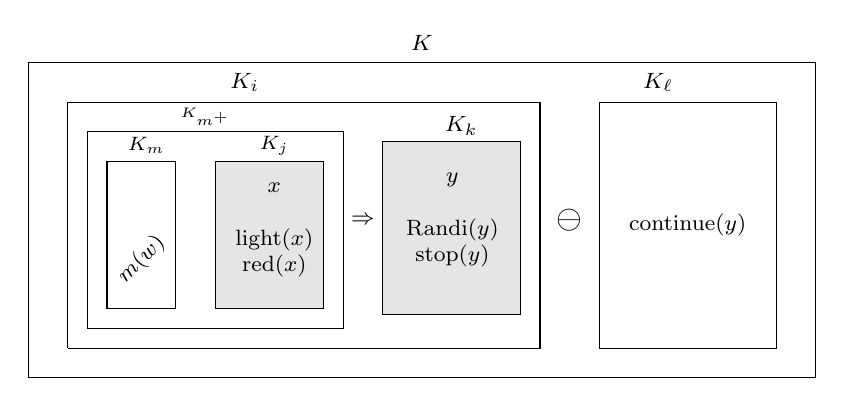
\begin{tikzpicture}\footnotesize
\draw (0,0) -- (10,0) -- (10,4) -- (0,4) -- (0,0);%Kbox
\draw (.5,.375) -- (6.5,.375) -- (6.5,3.5) -- (.5,3.5) -- (.5,.375);%Ki box
\draw (.75,.625) -- (4,.625) -- (4,3.125) -- (.75,3.125) -- (.75,.625);%Km+ box
\draw (1,.875) -- (1.875,.875) -- (1.875,2.75) -- (1,2.75) -- (1,.875);%Km box
\node[align=center,rotate=45] at (1.4375,1.5) {$m(w)$};%Kmtext
\draw[fill=gray!20] (2.375,.875) -- (3.75,.875) -- (3.75,2.75) -- (2.375,2.75) -- (2.375,.875);%Kj box
\node[align=center] at (3.125,1.875) {$x$\\\\ light($x$)\\red($x$)};%Kjtext
\draw[fill=gray!20] (4.5,.8) -- (6.25,.8) -- (6.25,3) -- (4.5,3) -- (4.5,.8);%Kk box
\node[align=center] at (5.3875,2) {$y$\\\\ Randi($y$)\\stop($y$)};%Kk txt
\draw (7.25,.375) -- (9.5,0.375) -- (9.5,3.5) -- (7.25,3.5) -- (7.25,0.375);%KL
\node[align=center] at (8.375,2) {\\ continue($y$)}; %\\$ z=y $		
\node[align=center] at (2.125,1.875) {{$\Cap$}}; %conditional op
\node[align=center] at (6.875,2) {{\large$\ominus$}}; %otherwise op
\node[align=center] at (4.25,2) {{$\boldsymbol\Rightarrow$}}; %cons op
%%
\node[align=center] at (5,4.25) {$ K $}	;
\node[align=center] at (2.75,3.75) {$\boldsymbol{K_i} $};
\node[align=center] at (2.25,3.3125) {{\tiny$\boldsymbol{ K_{m^+}} $}};
\node[align=center] at (1.5,2.95) {{\scriptsize$ \boldsymbol{K_m} $}};
\node[align=center] at (3.125,2.95) {{\scriptsize$ K_{j} $}};
\node[align=center] at (5.5,3.2) {$ K_k $};
\node[align=center] at (8,3.75) {$ K_\ell $};\\
\end{tikzpicture}
\-\\\vspace{1pt}
Where the following satisfaction conditions hold:
\begin{itemize}
  	\item \, $C_K = \{K_i\underset{m,o}{\ominus} K_\ell\}$
	\item \, $C_{K_i} =\{ K_j\, \underset{m,o}{\square}\, K_k\} = \{K_{m^+}\Rightarrow K_k	\}$
	%&C_{K_{m^+}}=\{\}\\
	\item  $C_{K_j} = \{\text{light}(x),\,\text{red}(x)\}$
	\item  $C_{K_k} = \{\text{Randi}(y), \text{stop}(y)\}$
	\item  $C_{K_\ell} = \{\text{continue}(y)\}$
	\item  $C_{K_m} = \{c\mid\langle w',f\rangle\Vdash c\} \text{ where } w'\in\underset{deo(w)}{\textsc{best}}\big(\cap\underset{\textsc{circ}}{m(w)}\big)$
	\item  $C_{K_{m^+}} = \{K_m\Cap K_j\} = \{c\mid\langle w''\!,f\rangle\Vdash c\} $
%where $w''\in\underset{deo(w)}{\textsc{best}}\big(\cap\big(\underset{\textsc{circ}}{m(w)}\cup\{w'''\mid\langle w'''\!\!,f\rangle\vDash K_j\}\big)\big) $
\end{itemize}
\a DRS illustration spelling out accommodation of the antecedent proposition $ (K_{i_{\text{sub}}}) $ (compare to \S \ref{sec:proposal}, esp. exx. \ref{redlight-Ki} \& \ref{antec-skel}):\\
\drs{~}{\hfill\xdrs{~~~$K_i$}\\$ \neg $\xdrs{~~~$ K_{m^+} $}$\square$\xdrs{~~~$ K_\ell $}}
\xe%

%\textcolor{red}{Josh: I changed a couple of the satisfaction conditions from what you had originally. Do you notice any issues there? }\textcolor{violet}{i don't thiiiink i do? do you remember what they were?}

With the satisfaction conditions we introduced above, we can construct the truth-conditions that will verify the matrix DRS $ K $: 

\pex \textit{Satisfaction conditions for \blastx:}
\a\uline{Simplex conditions:}\\ 
The DRSs $ K_j,K_k,K_\ell $ all contain only atomic conditions.\\ Each of these DRSs is verified iff there is some world-assignment pair $ \langle w,f\rangle $ which satisfies all of their respective conditions.\\
\begin{itemize}
	\item  $\langle w,f\rangle \vDash K_j \leftrightarrow \langle w,f\rangle \Vdash \text{red.light}(y) \leftrightarrow f(y)\in\Sem[w]{red.light}$\\
	\item   $\langle w,f\rangle \vDash K_k \leftrightarrow \langle w,f\rangle \Vdash \text{Randi}(y)\wedge \text{stop}(y) \leftrightarrow f(y)\in\Sem[w]{Randi}\cap\Sem[w]{stop}$\\
	\item   $\langle w,f\rangle \vDash K_\ell \leftrightarrow \langle w,f\rangle \Vdash \text{continue}(y) \leftrightarrow f(y)\in\Sem[w]{continue}$
\end{itemize}
\a \uline{The antecedent to \textit{otherwise} $ C_{K_i} $:}\\
The antecedent $ K_i $ is verified iff some world-assignment pair $ \langle w,f\rangle $ satisfies the (complex) condition $ K_j\,\square\,K_k $ :\\ 
%
$\langle w,f\rangle\Vdash (K_j\underset{m,o}{\square} K_k )\leftrightarrow \\
  	\forall w',g\big[g{\scriptscriptstyle\langle X_{K_j}\rangle}f \wedge w'\in\underset{tel(w)}{\textsc{best}}\big(\bigcap\big(\underset{\textsc{circ}}{m(w)}\cup\{w''\mid\langle w'',g\rangle\vDash K_j\}\big)\big) \to\\
	\hspace*{2.7em} \exists g''[g''{\scriptscriptstyle\langle X_{K_k}\rangle}g \wedge \langle w',g''\rangle\vDash K_k]\big]$\\[1em]
%
That is: $ \langle w,f\rangle\vDash K_i $ iff for all $ w' $ in a circumstantial modal base $ \underset{\textsc{circ}}{m(w)} $ that best conform to a teleological ordering source $ o_{tel}(w) $: if there is some assignment $g'$ that verifies $ K_j $ in $w'$, then there is some assignment $ g'' $ that verifies $ K_k $  in $w'$.
\a \uline{The matrix condition $ C_K $:}\\
A world-assignment pair $\langle  w,f \rangle$ verifies the entire DRS $ K $ iff it satisfies the (complex) condition $ K_i\ominus K_\ell $ : 
\label{Ck}\\
%
$\langle w,f\rangle \Vdash(K_i\underset{m',o'}{\ominus} K_\ell)\leftrightarrow\exists g[g{\scriptscriptstyle\langle X_{K_i}\rangle}f\wedge\langle w,g\rangle\vDash K_i] 
\;\wedge\\
\forall w',g'[g'{\scriptscriptstyle\langle X_{K_i}\rangle}f\wedge w'\in\underset{tel(w)}{\textsc{best}}\Big(\bigcap\big(\underset{\textsc{circ}}{m'(w)}\cup\{w''\mid\langle w'',g'\rangle\vDash(\neg K_{i_{\text{sub}}})\}\big)\Big) \to\\
	\hspace*{2.85em} \exists g''(g''{\scriptscriptstyle\langle X_{K_\ell}\rangle}g'\wedge \langle w',g''\rangle\vDash K_\ell)]$\\[1em]
%\end{multline*}
That is: $ \langle w,f\rangle\vDash K $ iff:
\begin{itemize}
	\item \; There is some assignment $ g $ that verifies $ K_i $ and
	\item \; If those worlds $ w' $ in a circumstantial modal base $\underset{\textsc{circ}}{m(w)}$ that best conform to a teleological ordering source (likely one that contains Randi's desires to both get where she needs to be and to be an upstanding road user) \textbf{verify the negation of} $ \boldsymbol{ K_{m^+}} $ (the antecedent to \textit{otherwise}, accommodated due to the processes described in \S\ref{sec:qud}), then there'll be some assignment $ g'' $ that verifies $ K_\ell $ in $w'$.
\end{itemize}
%
\xe
%\textcolor{red}{Josh, please add descriptions of these formulas (at least in a and b) in words. This is really hard to follow. Specifically, define $O_{tel}$, $m_{circ}$. What does this complex condition require?}

Notably, $ y $ is an unbound variable in its local DRS --- however, because $ K_i\leqslant K_\ell $, $ K_\ell $  has access to the local domain of this DRS $ (A_{K_\ell}\supseteq X_{K_{i}}) $. As a result, the assignment function ($ g'' $ in \ref{Ck} above) is able to assign to $ y $ an individual introduced earlier in the discourse (namely `Randi').
 We see, then, that our analysis is able to correctly model an \textit{otherwise} statement, making crucial use of the notion of modal subordination and other tools that foreground discourse dynamics to provide the truth conditions for the sentence. 
 
 
 
 
 




%\section*{Contact information}
%\vfill\noindent Josh Phillips, Hadas Kotek \\
%\noindent \texttt{josh.phillips@yale.edu}, \texttt{hkotek@alum.mit.edu}





